\documentclass[10pt,handout]{beamer} 
\PassOptionsToPackage{most}{tcolorbox}
\usetheme{jambro}
\tcbuselibrary{listings}
\graphicspath{{./Primer/graphics/}}
\usepackage{wasysym}
\hypersetup{colorlinks,citecolor=main,linkcolor=white,urlcolor=main}
\usepackage{newverbs}
\usepackage{courier}
 
% MATLAB code environments (matches handbook: matlabcode, matlaboutput)
% Note: frames containing matlabcode/matlaboutput must use \begin{frame}[fragile]
%-----------------------------------------------------
\makeatletter
\newcommand*\codesize{\@setfontsize\codesize{8.0}{9.5}}
\newcommand*\codesizebox{\@setfontsize\codesizebox{7.0}{8.5}}
\makeatother
% Inline monospace highlight, imported from handbook (VAR_Handbook.tex)
\newcommand{\mc}[1]{\colorbox{script!80}{\codesize\texttt{#1}}}
\definecolor{matlabbg}{RGB}{255,248,225}
\lstdefinestyle{matlab}{
language=Matlab,
basicstyle=\codesizebox\ttfamily,
keywordstyle=\color{matlabblue},
commentstyle=\color{matlabgreen},
stringstyle=\color{matlabpurple},
numberstyle=\tiny\color{gray},
numbers=none,
breaklines=true,
breakatwhitespace=true,
showstringspaces=false,
tabsize=4,
keepspaces=true,
columns=flexible,
frame=none,
backgroundcolor=\color{matlabbg},
xleftmargin=3pt,
xrightmargin=3pt,
aboveskip=0pt,
belowskip=0pt,
deletekeywords={detc,beta,sign,NaN,type,pi},
}
\lstset{style=matlab}
\newtcblisting{matlabcode}{
listing only,
listing options={style=matlab},
colback=script,
colframe=black!50,
boxrule=0.6pt,
arc=2pt,
left=3pt, right=3pt, top=3pt, bottom=3pt,
width=0.92\textwidth,          % slightly narrower so the box looks centered in a list
before={\par\vspace{6pt}\centering},
after={\par},
breakable,
}
\newenvironment{matlaboutput}
{\par\vspace{6pt}\codesize\ttfamily\Verbatim}
{\endVerbatim\par\vspace{6pt}\normalsize}

% Note box (matches handbook notebox: note!15 background, hand font header)
%-----------------------------------------------------
\definecolor{notebg}{RGB}{225,230,240}
\DeclareRobustCommand{\hand}{%
\fontfamily{augie}\fontseries{m}\fontshape{n}\selectfont}
\newcommand{\handdotfill}{%
\leavevmode\xleaders\hbox{{\hand\small ·}\,}\hfill\kern0pt}
% #1 = title (default: Note); #2 = extra tcolorbox options (e.g. height fill)
\newtcolorbox{notebox}[2][Note]{%
enhanced,
colback=notebg,  colframe=title,  boxrule=0.5pt,
left=6pt, right=6pt, top=4pt, bottom=6pt,
before upper={%
\noindent\handdotfill\enskip{\color{title}#1}\enskip\handdotfill\par\smallskip%
\sffamily\small},
#2
}
% Bottom spacer that shifts the (valign lower=center) body up by half the title
% strip, so the body's midpoint lands on the slide centre rather than on the
% centre of the space left below the title. Constant across boxes (single-line
% \large titles). Place just before the end of the box.
\newcommand{\noteboxcenter}{\vspace*{0.9cm}}

% Authors/institutes/date/etc
%-----------------------------------------------------
\title[VAR models]{\textbf{A Primer on Vector Autoregressions}}
\subtitle{VAR Toolbox 4.0}
\author[]{Ambrogio Cesa-Bianchi}
\date{\today}

\begin{document}

%=============================================================
\section{Introduction}
\begin{frame}[plain]
\titlepage
\end{frame}
%.......................................................
\shownotesblock{}

%=============================================================
\begin{frame}
\bigskip\bigskip
\begin{equation*}
\text{\textbf{[DISCLAIMER]}}
\end{equation*}
\bigskip \bigskip
\centering
\begin{minipage}{.8\textwidth}
These notes are meant to provide intuition on the basic mechanisms of VARs \par\bigskip
As such, most of the material covered here is treated in a very informal way \par\bigskip
If you crave a formal treatment of these topics, you should stop here and buy a copy of Hamilton's \textquotedblleft Time Series Analysis\textquotedblright \par\bigskip
The Matlab codes accompanying the notes are available at:\newline \url{https://github.com/ambropo/VAR-Toolbox}
\end{minipage}
\end{frame}
%.......................................................
\shownotesblock{}

%=============================================================
\begin{frame}
{The job of macro-econometricians}
\begin{itemize}
\item In their 2001 Journal of Economic Perspectives' article \textquotedblleft Vector Autoregressions\textquotedblright\ \cite{StockWatson2001} describe the job of macroeconometricians as consisting of the following tasks \smallskip
\begin{itemize}
\item Describe and summarize macroeconomic time series \smallskip
\item Make forecasts \smallskip
\item Recover the structure of the macroeconomy from the \lapis{data} \smallskip
\item Advise macroeconomic policy-makers\bigskip \pause \medskip
\end{itemize}
\item Vector autoregressive models (VARs) are a statistical tool to perform
these tasks
\end{itemize}
\end{frame}
%.......................................................
\shownotesblock{}

%=============================================================
\begin{frame}
{What can we do with VARs?}
\begin{itemize}
\item Consider an (over-simplistic) bivariate VAR\ with the following variables: \smallskip
\begin{itemize}
\item Real GDP growth ($y_{t}$) \smallskip
\item Policy rate ($r_{t}$)\bigskip \medskip \pause \medskip
\end{itemize}
\item A VAR\ can help us answer the following questions\smallskip
\begin{enumerate}
\item[{[1]}] What is the dynamic behavior of these variables? How do these variables interact?\medskip
\item[{[2]}] What is the most likely path of GDP in the next few quarters? \medskip
\item[{[3]}] What is the effect of a monetary policy shock on GDP?\medskip
\item[{[4]}] What has been the historical contribution of monetary policy shocks to GDP fluctuations?
\end{enumerate}
\end{itemize}
\end{frame}
%.......................................................
\shownotesblock{}

%=============================================================
\subsection{The Reduced-Form VAR}
\begin{frame}
\color{title} \centering{\huge \textbf{(S)VARs\ Basics}} \par\bigskip
\color{note} \centering{\Large \textbf{The Reduced-Form VAR}}
\end{frame}
%.......................................................
\shownotesblock{}

%=============================================================
\begin{frame}
{The reduced-form VAR}
\begin{itemize}
\item A VAR with $k$ endogenous variables and $p$ lags describes the evolution of the $k\times 1$ vector $x_t$ as a function of its own lags, a constant, and a serially uncorrelated error term
\begin{equation*}
x_{t}= c + \Phi_1 x_{t-1} + \cdots + \Phi_p x_{t-p} + u_{t}
\end{equation*}
\vspace{-.4cm}
\item where \smallskip
\begin{itemize}
\item $c$ is a $k\times 1$ vector of intercepts \smallskip
\item $\Phi_1,\ldots,\Phi_p$ are $k\times k$ matrices of autoregressive coefficients \smallskip
\item $u_t$ is a $k\times 1$ vector of serially uncorrelated reduced-form residuals with zero mean and time-invariant covariance matrix $\mathbb{V}(u_t)\equiv\Sigma_u$ (homoskedasticity) \medskip
\end{itemize}
\end{itemize}
\end{frame}
%.......................................................
\shownotesblock{}

%=============================================================
\begin{frame}
{A bivariate running example}
\begin{itemize}
\item The running example in this primer is a bivariate VAR(1) in $x_t=(y_t,r_t)'$, where \smallskip
\begin{itemize}
\item $y_t$ is the log difference of US real GDP \smallskip
\item $r_t$ is the 1-year US Treasury bill yield \medskip
\end{itemize}
\end{itemize}\pause
\begin{center}
\NB[0.9\textwidth]{\textbf{\hspace{4cm} \lapis[BoEred]{Warning: Do not try this at home!}} \\\medskip
\small
The bivariate VAR(1) used throughout is a purely pedagogical device. With only two variables and one lag, the algebra is tractable and the toolbox mechanics are easy to follow. But this is not a credible empirical model: no referee, advisor, or editor would accept it as serious applied work. Use it to understand how the toolbox works; do not use it as a template for research.}\smallskip\pause
\end{center}
\begin{itemize}
\item The reduced-form representation of this simple VAR(1) is\smallskip
\begin{equation*}
\begin{bmatrix} y_t \\ r_t \end{bmatrix}
= \begin{bmatrix} c_y \\ c_r \end{bmatrix}
+ \begin{bmatrix} \phi_{11} & \phi_{12} \\ \phi_{21} & \phi_{22} \end{bmatrix}
\begin{bmatrix} y_{t-1} \\ r_{t-1} \end{bmatrix}
+ \begin{bmatrix} u_{yt} \\ u_{rt} \end{bmatrix}
\end{equation*}
\end{itemize}
\end{frame}
%.......................................................
\shownotesblock{}

%=============================================================
\begin{frame}
{The reduced-form VAR}
\begin{itemize}
\item This formulation of the VAR is called the \lapis{\textbf{reduced-form VAR}}
representation
\begin{equation*}
x_{t}=c+\Phi x_{t-1}+u_{t}
\end{equation*}%
\pause
\item In matrix form%
\begin{equation*}
\begin{bmatrix}
y_{t} \\
r_{t}%
\end{bmatrix}%
=%
\begin{bmatrix}
c_y \\
c_r%
\end{bmatrix}%
+%
\begin{bmatrix}
\phi _{11} & \phi _{12} \\
\phi _{21} & \phi _{22}%
\end{bmatrix}%
\begin{bmatrix}
y_{t-1} \\
r_{t-1}%
\end{bmatrix}%
+%
\begin{bmatrix}
u_{yt} \\
u_{rt}%
\end{bmatrix}%
\medskip
\end{equation*}
\item Or as a system of linear equations%
\begin{equation*}
\left\{
\begin{array}{c}
y_{t}=c_y+\phi _{11}y_{t-1}+\phi _{12}r_{t-1}+u_{yt} \\
r_{t}=c_r+\phi _{21}y_{t-1}+\phi _{22}r_{t-1}+u_{rt}%
\end{array}%
\right.
\end{equation*}
\end{itemize}
\end{frame}
%.......................................................
\shownotesblock{}

%=============================================================
\begin{frame}
{The reduced-form covariance matrix}
\begin{itemize}
\item A key object of interest in VARs is the covariance matrix of the \lapis{\textbf{reduced-form residuals}}
\begin{equation*}
\Sigma_{u}\equiv \mathbb{E}\left[u_t u'_t\right] =\left[
\begin{array}{cc}
\sigma_{y}^{2} & \sigma_{yr} \\
\sigma_{yr} & \sigma_{r}^{2}%
\end{array}%
\right]
\end{equation*}
\item $\Sigma_u$ is symmetric (same off-diagonal elements $\sigma_{yr}$) and positive definite \bigskip
\item Typically, the reduced-form residuals are correlated among each other ($\sigma_{yr}\neq 0$)\bigskip
\item This is because the elements of $u_{t}$ inherit all the contemporaneous relations among the endogenous variables $x_{t}$\bigskip
\item Thus, we can't use $u_t$ to make causal statements about structural shocks hitting the economy \smallskip
\begin{itemize}
\item e.g. what are the effects of a monetary policy `shock' on output \medskip
\end{itemize}
\end{itemize}
\end{frame}
%.......................................................
\shownotesblock{}

%=============================================================
\subsection{The Structural VAR Representation}
\begin{frame}
\color{title} \centering{\huge \textbf{(S)VARs\ Basics}} \par\bigskip
\color{note} \centering{\Large \textbf{The Structural VAR Representation}}
\end{frame}
%.......................................................
\shownotesblock{}

%=============================================================
\begin{frame}
{The structural VAR representation}
\begin{itemize}
\item Let the only two structural shocks be a demand and a monetary policy shock \bigskip
\item The reduced-form VAR(1) above can be written in its \lapis{\textbf{structural form}} as:
\begin{equation*}
\begin{bmatrix}
y_{t} \\
r_{t}%
\end{bmatrix}%
=%
\begin{bmatrix}
c_{y} \\
c_{r}
\end{bmatrix}%
+
\begin{bmatrix}
\phi _{11} & \phi _{12} \\
\phi _{21} & \phi _{22}%
\end{bmatrix}%
\begin{bmatrix}
y_{t-1} \\
r_{t-1}%
\end{bmatrix}%
+%
\begin{bmatrix}
b_{11} & b_{12} \\
b_{21} & b_{22}%
\end{bmatrix}%
\begin{bmatrix}
\varepsilon_{t}^{Demand} \\
\varepsilon_{t}^{MonPol}%
\end{bmatrix}%
\end{equation*}%
\smallskip
\item The \lapis{\textbf{structural shocks}} $\varepsilon_t$ have a well-defined economic interpretation
\smallskip
\begin{itemize}
\item Serially uncorrelated, mutually uncorrelated, with zero mean and unit variance: $\mathbb{E}[\varepsilon_t]=0$, $\mathbb{E}[\varepsilon_t\varepsilon_t']=I_2$ \medskip
\end{itemize}
\item The \lapis{\textbf{structural impact matrix}}  $B$ maps structural shocks into the variables \smallskip
\begin{itemize}
\item The $(i,j)$ element of $B$ is the \textit{impact} response of variable $i$ to shock $j$ \medskip
\end{itemize}\pause \bigskip
\item The structural and reduced-form VAR are linked by $u_t = B\varepsilon_t$, so that 
\begin{equation*}
\Sigma_{u}=\mathbb{E}\left[ u_{t}u_{t}^{\prime}\right] =\mathbb{E}\left[B\varepsilon_{t}\left( B\varepsilon_{t}\right) ^{\prime}\right] =B\mathbb{E}(\varepsilon_{t}\varepsilon_{t}^{\prime})B^{\prime}=B\Sigma_{\varepsilon }B^{\prime}=BB^{\prime}
\end{equation*}
\end{itemize}
\end{frame}
%.......................................................
\shownotesblock{}

%=============================================================
\begin{frame}
{Three different ways of writing the same thing}
\begin{itemize}
\item There are different ways to write the same structural VAR(1)
\begin{equation*}
x_{t}=c+\Phi x_{t-1}+B\varepsilon_{t}
\end{equation*}%
\pause\vspace{-0.3cm}
\item For example, we can write it in matrix form%
\begin{equation*}
\begin{bmatrix}
y_{t} \\
r_{t}%
\end{bmatrix}%
=%
\begin{bmatrix}
c_{y} \\
c_{r}%
\end{bmatrix}%
+%
\begin{bmatrix}
\phi _{11} & \phi _{12} \\
\phi _{21} & \phi _{22}%
\end{bmatrix}%
\begin{bmatrix}
y_{t-1} \\
r_{t-1}%
\end{bmatrix}%
+%
\begin{bmatrix}
b_{11} & b_{12} \\
b_{21} & b_{22}%
\end{bmatrix}%
\begin{bmatrix}
\varepsilon_{t}^{Demand} \\
\varepsilon_{t}^{MonPol}%
\end{bmatrix}%
\end{equation*}%
\pause
\item Or as a system of linear equations%
\begin{equation*}
\left\{
\begin{array}{l}
y_{t}=c_y+\phi _{11}y_{t-1}+\phi _{12}r_{t-1}+b_{11}\varepsilon_{t}^{Demand}+b_{12}\varepsilon_{t}^{MonPol}\smallskip \\
r_{t}=c_r+\phi _{21}y_{t-1}+\phi _{22}r_{t-1}+b_{21}\varepsilon_{t}^{Demand}+b_{22}\varepsilon_{t}^{MonPol}%
\end{array}%
\right.
\end{equation*}
\end{itemize}
\end{frame}
%.......................................................
\shownotesblock{}

%=============================================================
\begin{frame}
{Why reduced-form residuals are correlated}
\begin{itemize}
\item Now that we have introduced the structural shocks $\varepsilon_t$, we can explain why $\Sigma_u$ typically has non-zero off-diagonal elements\bigskip\pause
\item The reduced-form residuals $u_t$ are \textbf{mixtures} of structural shocks: $u_t = B\varepsilon_t$, so\smallskip
\begin{equation*}
\left\{
\begin{array}{l}
u_{yt}=b_{11}\varepsilon_{t}^{Demand}+b_{12}\varepsilon_{t}^{MonPol} \\
u_{rt}=b_{21}\varepsilon_{t}^{Demand}+b_{22}\varepsilon_{t}^{MonPol}%
\end{array}%
\right.
\end{equation*}\pause
\item Although structural shocks are orthogonal ($\mathbb{E}[\varepsilon_t\varepsilon_t']=I_2$), the reduced-form residuals are correlated because they share the same underlying shocks
\end{itemize}
\end{frame}
%.......................................................
\shownotesblock{}

%=============================================================
\begin{frame}
{Why is it called `structural' VAR?}
\begin{itemize}
\item Go back to our bivariate structural VAR(1)
\begin{equation*}
\begin{bmatrix}
y_{t} \\
r_{t}%
\end{bmatrix}%
=%
\begin{bmatrix}
c_{y} \\
c_{r}%
\end{bmatrix}%
+%
\begin{bmatrix}
\phi _{11} & \phi _{12} \\
\phi _{21} & \phi _{22}%
\end{bmatrix}%
\begin{bmatrix}
y_{t-1} \\
r_{t-1}%
\end{bmatrix}%
+%
\begin{bmatrix}
b_{11} & b_{12} \\
b_{21} & b_{22}%
\end{bmatrix}%
\begin{bmatrix}
\varepsilon_{t}^{Demand} \\
\varepsilon_{t}^{MonPol}%
\end{bmatrix}%
\end{equation*}
\item The structural VAR\ can be thought of as a description of the true structure of the economy \smallskip
\begin{itemize}
\item e.g.\ an approximation of the solution of a DSGE\ model \medskip
\end{itemize}
\item The structural shocks are shocks with a well-defined economic interpretation \smallskip
\begin{itemize}
\item e.g.\ TFP\ shocks or monetary policy shocks \smallskip
\item Since the structural shocks are mutually uncorrelated, we can move one shock keeping the other shocks fixed \smallskip
\item That is:\ we can focus on the causal effect of one shock at the time \medskip
\end{itemize}
\end{itemize}
\end{frame}
%.......................................................
\shownotesblock{}

%=============================================================
\begin{frame}
{Structural VARs can answer many interesting questions...}
\begin{itemize}
\item Go back to our bivariate structural VAR(1), and assume for the moment that $\Phi$ and $B$ are known \bigskip
\item In matrix form:
\begin{equation*}
\begin{bmatrix}
y_{t} \\
r_{t}%
\end{bmatrix}%
=%
\begin{bmatrix}
c_{y} \\
c_{r}%
\end{bmatrix}%
+{\tikz[tstyle]{\node[nstyle](node0){$\begin{bmatrix} \phi _{11} & \phi _{12} \\ \phi _{21} & \phi _{22}\end{bmatrix}$};}}
\begin{bmatrix}
y_{t-1} \\
r_{t-1}%
\end{bmatrix}%
+{\tikz[tstyle]{\node[nstyle](node1){$\begin{bmatrix} b_{11} & b_{12} \\ b_{21} & b_{22}\end{bmatrix}$};}}
\begin{bmatrix}
\varepsilon_{t}^{Demand} \\
\varepsilon_{t}^{MonPol}%
\end{bmatrix}%
\end{equation*}%
\vspace{-0.15cm} \medskip \pause

\item What is the effect of monetary policy shocks on output?\smallskip\pause \smallskip

\begin{itemize}
\item The coefficient $b_{12}$ captures the `impact effect' of a monetary
policy shock on output growth\medskip 
\begin{tikzpicture}[tpstyle]
\node[pencil,draw, minimum height=1.2cm, minimum width=1.7cm] (box1) at (node1) {};
\draw[arrow,->,opacity=1] (box1.north) to[bend left] +(+0.9,0.4) node[gold,anchor=west,opacity=1] {\footnotesize{\textbf{\hand Impact matrix}}};
\end{tikzpicture}
\pause \smallskip

\item The $\Phi $ matrix allows us to trace the `dynamic effect' of the
monetary policy shock over time\medskip 
\begin{tikzpicture}[tpstyle]
\node[pencil,draw, minimum height=1.2cm, minimum width=1.7cm] (box0) at (node0) {};
\draw[arrow,->,opacity=1] (box0.north) to[bend right] +(-0.9,0.2) node[gold,anchor=east,opacity=1] {\footnotesize{\textbf{\hand Dynamic matrix}}};
\end{tikzpicture}
\pause \smallskip

\item (We can add additional variables and look at other shocks: aggregate
supply, oil price,...) \medskip
\end{itemize}
\end{itemize}
\end{frame}
%.......................................................
\shownotesblock{}

%=============================================================
\begin{frame}
{... but the estimation of structural VARs is tricky}
\begin{itemize}
\item \textbf{Problem} \ The structural shocks $\varepsilon_{t}$ are unobserved. So, how can we estimate $B$?
\begin{equation*}
\begin{bmatrix}
y_{t} \\
r_{t}%
\end{bmatrix}%
=%
\begin{bmatrix}
c_{y} \\
c_{r}%
\end{bmatrix}%
+%
\begin{bmatrix}
\phi _{11} & \phi _{12} \\
\phi _{21} & \phi _{22}%
\end{bmatrix}%
\begin{bmatrix}
y_{t-1} \\
r_{t-1}%
\end{bmatrix}%
+%
\begin{bmatrix}
b_{11} & b_{12} \\
b_{21} & b_{22}%
\end{bmatrix}%
\begin{bmatrix}
\varepsilon_{t}^{Demand} \\
\varepsilon_{t}^{MonPol}%
\end{bmatrix}%
\end{equation*}%
\pause

\item Best we can do is to `bundle' the $\varepsilon_{t}$ into a single
object: 
\begin{equation*}
u_{t}=B\varepsilon_{t}\Rightarrow 
\begin{bmatrix}
u_{yt} \\ 
u_{rt}
\end{bmatrix}%
=
\left[ 
\begin{array}{cc}
b_{11} & b_{12} \\ 
b_{21} & b_{22}%
\end{array}%
\right] 
\begin{bmatrix}
\varepsilon_{t}^{Demand} \\ 
\varepsilon_{t}^{MonPol}%
\end{bmatrix}%
\Rightarrow \left\{ 
\begin{array}{c}
u_{yt}=b_{11}\varepsilon_{t}^{Demand}+b_{12}\varepsilon_{t}^{MonPol} \\ 
u_{rt}=b_{21}\varepsilon_{t}^{Demand}+b_{22}\varepsilon_{t}^{MonPol}%
\end{array}%
\right.
\end{equation*}
\pause

\item Why is this useful?\ The VAR\ becomes%
\begin{equation*}
x_{t}=c+\Phi x_{t-1}+u_{t}
\end{equation*}%
\vspace{-.3cm}

\item Now we can estimate $\Phi $ and $u_{t}$ with OLS\ (where $u_{t}$ will
be OLS residuals)
\end{itemize}
\end{frame}
%.......................................................
\shownotesblock{}

%=============================================================
\subsection{The Wold Representation \& Stability}
\begin{frame}
\color{title} \centering{\huge \textbf{(S)VARs\ Basics}} \par\bigskip
\color{note} \centering{\Large \textbf{Wold Representations \& Stability}}
\end{frame}
%.......................................................
\shownotesblock{}

%=============================================================
\begin{frame}
{The Wold representation}
\begin{itemize}
\item Let's introduce another representation of the VAR\ that will be useful later
\bigskip
\item Start from the structural VAR\ representation
\begin{equation*}
x_{t}=c+\Phi x_{t-1}+B\varepsilon_{t}
\end{equation*}%
\vspace{-.45cm} \pause
\item The \lapis{\textbf{Wold representation}} can be obtained by substituting the VAR recursively
\begin{equation*}
\begin{array}{lll}
x_{t} & = & c+\Phi x_{t-1}+B\varepsilon_{t} \\ \medskip
\pause & = & c+\Phi \left( {\tikz[tstyle]{\node[nstyle](node1){$c+\Phi x_{t-2}+B\varepsilon_{t-1}$};}}\right) +B\varepsilon_{t}
\begin{tikzpicture}[tpstyle] \node[pencil,draw, minimum height=0.6cm, minimum width=3cm] (box1) at (node1) {}; \draw[arrow,->,opacity=1] (box1.south) to[bend right] +(+0.9,-0.2) node[gold,anchor=west,opacity=1] {\footnotesize{\textbf{\hand x\tiny{t-1}}}}; \end{tikzpicture}\pause
=(I+\Phi)c+\Phi ^{2}x_{t-2}+\Phi B\varepsilon_{t-1}+B\varepsilon_{t} \\
& = & ... \\
& = & \Phi ^{t}x_{0}+\sum\limits_{j=0}^{t-1}\Phi ^{j}c+\sum\limits_{j=0}^{t-1}\Phi ^{j}B\varepsilon_{t-j}%
\end{array}%
\end{equation*}
\end{itemize}
\end{frame}
%.......................................................
\shownotesblock{}

%=============================================================
\begin{frame}
{The Wold representation}
\begin{itemize}
\item The Wold representation shows that each observation ($x_{t}$) can be re-written as a combination of three terms \medskip
\begin{equation*}
x_{t}={\tikz[tstyle]{\node[nstyle](node1){$\Phi ^{t}x_{0}$};}}+{%
\tikz[tstyle]{\node[nstyle](node3){$\sum\limits_{j=0}^{t-1}\Phi^{j}c$};}}+{%
\tikz[tstyle]{\node[nstyle](node2){$\sum\limits_{j=0}^{t-1}\Phi
^{j}B\varepsilon_{t-j}$};}}
\end{equation*}%
\smallskip
\pause \smallskip
\begin{itemize}
\item An initial condition \medskip
\begin{tikzpicture}[tpstyle]
\node[pencil,draw, minimum height=0.55cm, minimum width=0.9cm] (box1) at (node1) {};
\draw[arrow,->,opacity=1] (box1.south) to[bend left] +(-0.9,-0.2) node[gold,anchor=east,opacity=1] {\footnotesize{\textbf{\hand Initial condition}}};
\end{tikzpicture}
\pause \smallskip
\item The cumulative contribution of the constant \medskip
\begin{tikzpicture}[tpstyle]
\node[pencil,draw, minimum height=1.3cm, minimum width=1.2cm] (box3) at (node3) {};
\draw[arrow,->,opacity=1] (box3.south) to[bend right] +(+0.8,-0.6) node[gold,anchor=west,opacity=1] {\footnotesize{\textbf{\hand Constant contribution}}};
\end{tikzpicture}
\pause \smallskip
\item The sum of current and past structural shocks \medskip
\begin{tikzpicture}[tpstyle]
\node[pencil,draw, minimum height=1.2cm, minimum width=1.8cm] (box2) at (node2) {};
\draw[arrow,->,opacity=1] (box2.east) to[bend left] +(+0.9,-0.3) node[gold,anchor=north west,opacity=1] {\footnotesize{\textbf{\hand Current \& past shocks}}};
\end{tikzpicture} \medskip
\end{itemize}
\medskip\pause
\item Now let $t\rightarrow \infty $ to get
\begin{equation*}
x_{t}=\Phi ^{\infty }x_{t-\infty }+\sum\limits_{j=0}^{\infty }\Phi^{j}c+\sum\limits_{j=0}^{\infty }\Phi
^{j}B\varepsilon_{t-j}
\end{equation*}
\pause
\item Matrix $\Phi$ plays a crucial role $\rightarrow$ Determines whether a shock from the infinitely distant past still has an effect on $x_t$ today
\end{itemize}
\end{frame}
%.......................................................
\shownotesblock{}

%=============================================================
\begin{frame}
{VAR stability}
\begin{itemize}
\item VARs are typically designed to study cyclical variations around trends \smallskip
\begin{itemize}
\item The effect of shocks progressively dissipate over time \medskip
\end{itemize}
\item Stability is the formal expression of this idea. For this to happen, two conditions must hold: \smallskip
\begin{itemize}
\item The infinite sums $\sum_{j=0}^{\infty}\Phi^{j}$ must converge to finite values \smallskip
\item The first term $\Phi^{\infty}x_{t-\infty}$ must vanish \medskip
\end{itemize}
\item \textbf{Mathematically} \ A\ VAR\ is called stable iff all the eigenvalues of $\Phi $ are less than $1$ in modulus.\pause\newline More formally: 
\begin{equation*}
\det \left( \Phi -\lambda I_{2}\right) =0\ \ \ \left\vert \lambda
\right\vert <1
\end{equation*}%
\pause
\item \textbf{Implication} \ In the absence of shocks, the VAR\ will converge to its equilibrium
\end{itemize}
\end{frame} 

\begin{frame}
\centering
\begin{notebox}[\large \handbold{[BOX]}  \ \textbf{Why eigenvalues govern stability?}]{height fill, valign lower=center, segmentation style={draw=notebg}, enlarge left by=-0.25cm, enlarge top by=0.1cm, enlarge bottom by=0.1cm}
\tcblower
\begin{itemize}
\item \textbf{Scalar case} \smallskip
\begin{itemize}
\item Suppose $x_t = \phi\, x_{t-1}$. After $j$ periods, $x_t = \phi^j x_0$ --- a geometric series \smallskip
\item Converges to zero if $|\phi|<1$; diverges if $|\phi|>1$ \smallskip
\item The scalar $\phi$ encodes all persistence in a single number\medskip
\end{itemize}
\item \textbf{VAR case} \smallskip
\begin{itemize}
\item The matrix $\Phi$ has $k$ eigenvalues $\lambda_1,\ldots,\lambda_k$ (solutions to $\det(\Phi - \lambda I)=0$) \smallskip
\item Raising to the $j$-th power: $\Phi^j = P\,\mathrm{diag}(\lambda_1^j,\ldots,\lambda_k^j)\,P^{-1}$ --- a geometric series running independently along each eigenvalue direction \smallskip
\item Converges to zero iff $|\lambda_i|<1$ for all $i$\medskip
\end{itemize}
\item \textbf{Key insight} \smallskip
\begin{itemize}
\item The largest eigenvalue in modulus governs how slowly the system returns to equilibrium \smallskip
\item Eigenvalue close to $1$ $\Rightarrow$ highly persistent responses \smallskip
\item Eigenvalue close to $0$ $\Rightarrow$ rapid decay
\end{itemize}
\end{itemize}
\end{notebox}
\end{frame}
%.......................................................
\shownotesblock{}

%=============================================================
\begin{frame}
{Equilibrium (the unconditional mean)}
\begin{itemize}
\item Start from an arbitrary $x_0$ (say because a shock pushed the system away from equilibrium) \bigskip
\item Where will $x_t$ be in the infinitely distant future? From the $h$-step-ahead Wold representation
\begin{equation*}
\mathbb{E}\left[x_{h}\mid x_0\right]
=\Phi^{h}x_{0}
\;+\;\sum_{j=0}^{h-1}\Phi^{j}c
\;+\;\sum_{j=0}^{h-1}\Phi^{j}B\,\mathbb{E}[\varepsilon_{h-j}]
\end{equation*}\pause
\item Under stability, as $h\to\infty$ only the constant terms survive:\medskip
\begin{equation*}
\lim_{h\to\infty}\,\mathbb{E}\left[x_{h}\mid x_0\right]
=\sum_{j=0}^{\infty}\Phi^{j}c
={\tikz[tstyle]{\node[nstyle](node1){$(I_{2}-\Phi)^{-1}$};}}c
\;\equiv\;\mu
\end{equation*}
\begin{tikzpicture}[tpstyle]
\node[pencil,draw, minimum height=0.8cm, minimum width=1.6cm] (box2) at (node1) {};
\draw[arrow,->,opacity=1] (box2.north east) to[bend left] +(+0.9,+0.1) node[gold,anchor=west,opacity=1] {\footnotesize{\textbf{\hand Geometric series}}};
\end{tikzpicture}\pause
\item The equilibrium the VAR converges to is the unconditional mean $\mu=(I-\Phi)^{-1}c$ 
\end{itemize}
\end{frame}


%------------------------------------------
\subsection{The Identification Problem}
%------------------------------------------

%=============================================================
\begin{frame}
\color{title} \centering{\huge \textbf{(S)VARs\ Basics}} \par\bigskip 
\color{note} \centering{\Large \textbf{The Identification Problem}}
\end{frame}


\begin{frame}
{Back to our reduced-form VAR}
\begin{itemize}
\item We have seen above that with OLS we can only estimate the reduced-form VAR\ (and not the structural VAR) \bigskip
\item Assume we already have an OLS estimate of $\hat{\Phi}$ and $\hat{u}_{t} $:%
\begin{equation*}
\begin{bmatrix}
y_{t} \\ 
r_{t}%
\end{bmatrix}%
=
\begin{bmatrix}
c_{y} \\
c_{r}%
\end{bmatrix}%
+%
\left[ 
\begin{array}{cc}
\phi _{11} & \phi _{12} \\ 
\phi _{21} & \phi _{22}%
\end{array}%
\right] 
\begin{bmatrix}
y_{t-1} \\ 
r_{t-1}%
\end{bmatrix}%
+%
\begin{bmatrix}
u_{yt}\\ 
u_{rt}%
\end{bmatrix}%
\medskip
\end{equation*}%
\pause
\item \textbf{Question} \ What is the effect of a monetary policy shock on GDP growth?\bigskip\pause
\item Unfortunately, the reduced-form innovations ($u_{yt}$ or $u_{rt}$) are not going to help us in answering the question
\end{itemize}
\end{frame}
%.......................................................
\shownotesblock{}

%=============================================================
\begin{frame}[t]
{Reduced-form VARs do not tell us anything about causality}
\begin{itemize}
\item To see that, recall we assumed that the `true' (and unobserved)\ model of the economy is%
\begin{equation*}
\begin{bmatrix}
y_{t} \\
r_{t}%
\end{bmatrix}%
=%
\begin{bmatrix}
c_{y} \\
c_{r}%
\end{bmatrix}%
+%
\begin{bmatrix}
\phi _{11} & \phi _{12} \\
\phi _{21} & \phi _{22}%
\end{bmatrix}%
\begin{bmatrix}
y_{t-1} \\
r_{t-1}%
\end{bmatrix}%
+%
\begin{bmatrix}
b_{11} & b_{12} \\
b_{21} & b_{22}%
\end{bmatrix}%
\begin{bmatrix}
\varepsilon_{t}^{Demand} \\
\varepsilon_{t}^{MonPol}%
\end{bmatrix}%
\end{equation*}
\pause
\item Also recall that the reduced-form innovations are a linear combination of the structural shocks
\begin{equation*}
\begin{array}{c}
u_{yt}=b_{11}\varepsilon_{t}^{Demand}+b_{12}\varepsilon_{t}^{MonPol}{%
\mathbf{\medskip }} \\ 
u_{rt}=b_{21}\varepsilon_{t}^{Demand}+b_{22}\varepsilon_{t}^{MonPol}%
\end{array}%
\end{equation*}%
\pause
\item An increase in $u_{rt}$ \lapis{is not a monetary policy shock}! could be due to \smallskip
\begin{itemize}
\item[{[1]}] A positive demand shock that increases both output growth and the policy rate \smallskip
\item[{[2]}] Or a monetary policy shock that decreases output growth and increases the policy rate \medskip
\end{itemize}
\pause
\item How to know whether it is {\small \color{title}[1]} or {\small\color{title}[2]}? This is the very nature of the \textbf{identification problem}!
\end{itemize}
\end{frame}
%.......................................................
\shownotesblock{}

%=============================================================
\begin{frame}
{The identification problem}
\begin{itemize}
\item The identification problem consists in finding a mapping from the reduced-form VAR\ to its structural counterpart%
\begin{equation*}
u_{t}= B\varepsilon_{t}
\end{equation*}
\pause
\item To do that, we can exploit the relation between reduced-form and structural innovations%
\begin{equation*}
\Sigma_{u}=BB^{\prime}
\end{equation*}
\item The identification problem simply boils down to finding a $B$ matrix that satisfies $\Sigma_{u}=BB^{\prime}$
\bigskip \pause
\item Unfortunately this is not as easy as it sounds. Why?
\smallskip
\begin{itemize}
\item Hint: There are infinite different $B$s that give you the same $\Sigma_{u}$ \medskip
\end{itemize}
\end{itemize}
\end{frame}
%.......................................................
\shownotesblock{}

%=============================================================
\begin{frame}
{The identification problem (cont'd)}
\begin{itemize}
\item Think of $\Sigma_{u}=BB^{\prime}$ as a system of equations 
\begin{equation*}
\left[ 
\begin{array}{cc}
\sigma_{y}^{2} & \sigma_{yr} \\ 
\sigma_{yr}  & \sigma_{r}^{2}%
\end{array}%
\right] =\left[ 
\begin{array}{cc}
b_{11} & b_{12} \\ 
b_{21} & b_{22}%
\end{array}%
\right] \left[ 
\begin{array}{cc}
b_{11} & b_{21} \\ 
b_{12} & b_{22}%
\end{array}%
\right]
\end{equation*}

\item Can be rewritten as%
\begin{equation*}
\left\{ 
\begin{array}{l}
\sigma_{y}^{2}=b_{11}^{2}+b_{12}^{2} \\ 
\sigma_{yr}=b_{11}b_{21}+b_{12}b_{22} \\ 
\sigma_{yr}=b_{11}b_{21}+b_{12}b_{22} \\ 
\sigma_{r}^{2}=b_{21}^{2}+b_{22}^{2}%
\end{array}%
\right.
\end{equation*}
\pause
\item \textbf{Problem} Because of the symmetry of $\Sigma_{u}$, the second and the third equation are identical!
\bigskip
\item We are left with $4$ unknowns (the elements of $B$) but only $3$ equations!
\end{itemize}
\end{frame}
%.......................................................
\shownotesblock{}

%=============================================================
\begin{frame}
\centering
\begin{notebox}[\large \handbold{[BOX]}  \ \textbf{The rotation representation of the identification problem}]{height fill, valign lower=center, segmentation style={draw=notebg}, enlarge left by=-0.25cm, enlarge top by=0.1cm, enlarge bottom by=0.1cm}
\tcblower
\begin{itemize}
\item Let $B_0$ be any matrix with $\Sigma_u = B_0 B_0'$ (e.g.\ the Cholesky factor). For any orthogonal $Q$ ($QQ'=I_k$), $B_0Q$ is \textit{also} a valid solution: $(B_0Q)(B_0Q)' = B_0\,QQ'\,B_0' = \Sigma_u$\bigskip
\item The set of \textit{all} solutions to $\Sigma_u=BB'$ is the orbit $\{B_0 Q : QQ'=I_k\}$. Every identification scheme is just a rule for selecting one particular $Q$\bigskip
\item In the bivariate case, $Q(\theta)=\left[\begin{smallmatrix}\cos\theta & -\sin\theta \\ \sin\theta & \cos\theta\end{smallmatrix}\right]$ is a plane rotation: the angle $\theta$ is the single free parameter left unconstrained by the 3 equations of $\Sigma_u=BB'$\bigskip
\item \textbf{Geometric intuition} \ The data pin down the \textit{shape} of the residual covariance ellipse, but not the \textit{directions} of the structural axes within it. Identification amounts to anchoring those directions
\end{itemize}
\noteboxcenter
\end{notebox}
\end{frame}
%.......................................................
\shownotesblock{}

%=============================================================
\section{Estimation}
\begin{frame}
\color{title} \centering{\huge \textbf{Estimation}}
\end{frame}
%.......................................................
\shownotesblock{}


%=============================================================
\begin{frame}[fragile]
{Adding the VAR Toolbox path to Matlab}
\begin{itemize}
\item To avoid clashes with functions from other toolboxes, add and remove the toolbox at the beginning and end of your scripts\bigskip
\item If you clone or download the toolbox to a folder named \texttt{VARToolbox}, add each subfolder explicitly to be safer: \par\smallskip
\begin{matlabcode}
% Identify the toolbox root from this file's location (one up from Primer)
root = fileparts(fileparts(mfilename('fullpath')));

% Add each relevant subfolder explicitly
addpath(fullfile(root, 'VAR'));
addpath(fullfile(root, 'Figure'));
addpath(fullfile(root, 'Stats'));
addpath(fullfile(root, 'Utils'));
addpath(fullfile(root, 'Primer'));
addpath(fullfile(root, 'Auxiliary'));
disp('VAR Toolbox 4.0 path set.');
.
.
% Remove the toolbox from the path at the end of the script
rmpath(genpath(root))
\end{matlabcode}
\end{itemize}
\end{frame}
%.......................................................
\shownotesblock{}

%=============================================================
\begin{frame}
{A simple bivariate VAR\ model}
\begin{itemize}
\item Our first example will be a simple bivariate VAR as the one considered above \bigskip
\item US\ quarterly data from 1989:Q1 to 2019:Q4 on output growth ($y_{t}$) and the 1-year T-bill ($r_{t}$)\bigskip
\end{itemize}
\begin{figure}[h]
\centering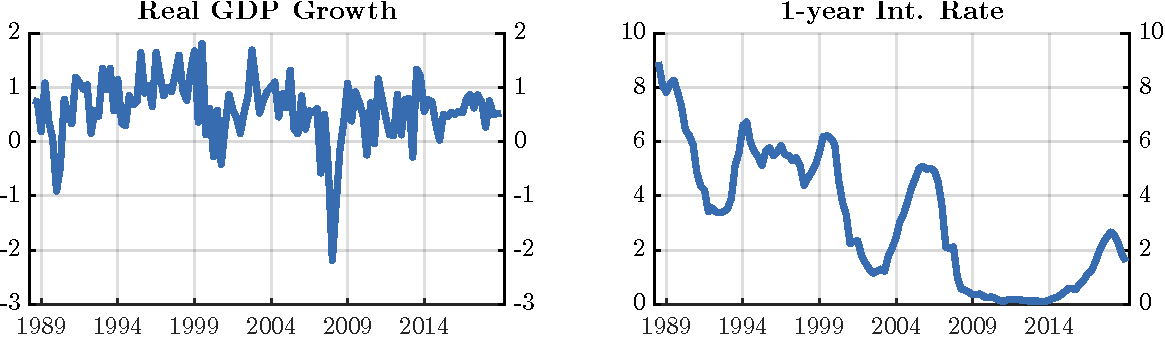
\includegraphics[width=.85\textwidth]{data.pdf}
\end{figure}
\end{frame}
%.......................................................
\shownotesblock{}

%=============================================================
\begin{frame}
{A simple bivariate VAR\ model}
\begin{itemize}
\item Fit GDP growth and the 1-year rate with a VAR(1) with a constant\medskip 
\begin{equation*}
\begin{bmatrix}
y_{t} \\ 
r_{t}%
\end{bmatrix}%
=%
\begin{bmatrix}
c_y \\ 
c_r%
\end{bmatrix}%
+\left[ 
\begin{array}{cc}
\phi _{11} & \phi _{12} \\ 
\phi _{21} & \phi _{22}%
\end{array}%
\right] 
\begin{bmatrix}
y_{t-1} \\ 
r_{t-1}%
\end{bmatrix}%
+%
\begin{bmatrix}
u_{yt}\\ 
u_{rt}%
\end{bmatrix}%
\end{equation*}%
\bigskip

\item This means we will estimate the following parameters \smallskip

\begin{itemize}
\item $2+4$ coefficients, namely the elements of $c $ and $\Phi $%
\smallskip

\item $2$ variances of the reduced-form residuals, namely $\sigma_{y}^{2}$
and $\sigma_{r}^{2}$ \smallskip

\item $1$ covariance of the reduced-form residuals, namely $\sigma_{yr}$%
\bigskip \medskip
\end{itemize}

\item We will store these coefficients in two Matlab matrices\medskip 
\begin{equation*}
\text{\mc{F}}=\left[ 
\begin{array}{ccc}
c_y & \phi _{11} & \phi _{12} \\ 
c_r & \phi _{21} & \phi _{22}%
\end{array}%
\right] \ \ \ \ \ \ \ \text{\mc{sigma}}=%
\left[ 
\begin{array}{cc}
\sigma_{y}^{2} & \sigma_{yr} \\ 
\sigma_{yr} & \sigma_{r}^{2}%
\end{array}%
\right]
\end{equation*}
\end{itemize}
\end{frame}
%.......................................................
\shownotesblock{}

%=============================================================
\begin{frame}[fragile]
{A simple bivariate VAR\ model}
\begin{itemize}
\item In Matlab we store the data in the matrix \mc{X}%
\begin{equation*}
\text{\mc{X}}=\left[ 
\begin{array}{cc}
y_{1} & r_{1} \\ 
y_{2} & r_{2} \\ 
... & ... \\ 
y_{T} & r_{T}%
\end{array}%
\right] \qquad \big(t\text{-th row: } x_{t}^{\prime}=(y_{t},\,r_{t})\big)
\end{equation*}
\item The VAR\ can then be easily estimated with a few lines of code \par\smallskip
\begin{matlabcode}
% Align variables to a common sample by removing leading/trailing NaNs
[X, fo, lo] = CommonSample(X);
% Initialise VAR options
VARopt = VARoption;
% Deterministic component: 1=constant, 2=constant+trend
detc = 1;
% Lag order
nlags = 1;
% Estimate VAR by OLS (reduced form only)
VAR_redform = VARmodel(X,nlags,detc,VARopt);
\end{matlabcode}
\end{itemize}
\end{frame}
%.......................................................
\shownotesblock{}

%=============================================================
\begin{frame}
{The \mc{VARopt} and \mc{VAR\_redform} structures}
\begin{itemize}
\item The \mc{VARopt} structure stores all the options and settings that control estimation and identification: \smallskip
\begin{itemize}
\item Created by \mc{VARoption} with sensible defaults for every field \smallskip
\item Includes identification scheme (\mc{ident}), number of horizons (\mc{nsteps}), variable names (\mc{vnames}) \smallskip
\item Can be reused and modified across multiple calls to \mc{VARmodel} and related functions \bigskip
\end{itemize}
\item The \mc{VAR\_redform} structure stores all the results of the VAR estimation \smallskip
\begin{itemize}
\item Includes reduced-form coefficients (\mc{F}), residuals (\mc{resid}), covariance matrix (\mc{sigma}), eigenvalues (\mc{maxEig}) \smallskip
\item Also includes identification results (once computed, not done here yet): $B$ matrix, impulse responses (\mc{IR}), variance decomposition (\mc{VD}), etc. \smallskip
\item Contains the input data: the endogenous variables (\mc{ENDO}), number of lags (\mc{nlag}), etc. \medskip
\end{itemize}
\end{itemize}
\end{frame}
%.......................................................
\shownotesblock{}

%=============================================================
\begin{frame}[fragile]
\frametitle{VAR\ output}
\begin{itemize}
\item The six estimated parameters (i.e. $c $ and $\Phi $)\ can be printed at screen by simply typing \mc{disp(VAR\_redform.F)} to get \par\smallskip
\begin{matlaboutput}
>> disp(VAR_redform.F)

0.3630    0.3788    0.0041
-0.0729    0.2607    0.9541
\end{matlaboutput}
\medskip
\item For the estimated reduced-form covariance matrix $\Sigma_{u}$ type \mc{disp(VAR\_redform.sigma)} \par\smallskip
\begin{matlaboutput}
>> disp(VAR_redform.sigma)

0.2891    0.0782
0.0782    0.1473
\end{matlaboutput}
\end{itemize}
\end{frame}
%.......................................................
\shownotesblock{}

%=============================================================
\begin{frame}
{OLS\ estimation: Typical VAR\ output (cont'd)}
\begin{itemize}
\item The off-diagonal elements of $\Sigma $ capture the \lapis{\textbf{average}} contemporaneous
relation between the endogenous variables \medskip

\begin{table}[tbph]
\centering%
\begin{tabular}{rrr}
\toprule & GDP growth ($u_{y}$) & 1-year T-bill ($u_{r}$) \\ 
\midrule GDP growth ($u_{y}$) & 0.2891 & {\tikz[tstyle]{%
\node[nstyle](node1){0.0782};}} \\
1-year T-bill ($u_{r}$) & 0.0782 & 0.1473 \\
\bottomrule &  & 
\end{tabular}%
\end{table}
\pause

\begin{tikzpicture}[tpstyle]
\node[pencil,draw, minimum height=0.5cm, minimum width=1.1cm] (box1) at (node1) {};
\draw[arrow,->,opacity=1] (box1.east) to[bend left] +(0.9,-0.1) node[gold,anchor=west,opacity=1] {\footnotesize{\textbf{\hand Cov(u\tiny{y}\footnotesize,u\tiny{r}\footnotesize)>0}}};
\end{tikzpicture}

\item In our example output growth and interest rates are contemporaneously positively correlated \smallskip

\begin{itemize}
\item It means that, on average, when GDP growth increases interest rates increase, too\bigskip \pause \medskip
\end{itemize}

\item Does it mean that a shock to interest rates always increases output growth? \smallskip

\begin{itemize}
\item No! Recall that reduced-form residuals are not informative about structural shocks \medskip
\end{itemize}
\end{itemize}
\end{frame}
%.......................................................



%=============================================================
\begin{frame}
{Model checking \& tuning}
\begin{itemize}
\item These notes do not cover this aspect in detail but... \bigskip
\item ... before interpreting the VAR results you should check a number of assumptions\bigskip \pause
\item Loosely speaking, you need to check that the reduced-form residuals are \smallskip
\begin{itemize}
\item Normally distributed \smallskip
\item Not autocorrelated \smallskip
\item Not heteroskedastic (i.e. have constant variance)\bigskip \pause \medskip
\end{itemize}
\item ... and that the VAR is stable (next slide)
\end{itemize}
\end{frame}
%.......................................................
\shownotesblock{}


%=============================================================
\begin{frame}[fragile]
\frametitle{Stability and equilibrium}
\begin{itemize}
\item We've already seen that a VAR\ is stable when all eigenvalues of its companion matrix lie inside the unit circle (for the VAR(1) here, the companion matrix is $\Phi$) \smallskip
\begin{itemize}
\item If this condition is not met, the infinite sums in the Wold representation do not converge \medskip
\end{itemize}
\pause
\item You can check the maximum modulus of the companion matrix's eigenvalues in the \mc{VAR} structure, by typing \mc{disp(VAR\_redform.maxEig)} to get \par\smallskip
\begin{matlaboutput}
>> disp(VAR_redform.maxEig)

0.9559
\end{matlaboutput}
\pause\medskip
\item You can also check all of the companion matrix's eigenvalues by executing Matlab's \mc{eig} function on \mc{Fcomp} (which, note, is built excluding the constant $c$ from \mc{F})\bigskip
\item In practice: \par\smallskip
\begin{matlaboutput}
>> disp(eig(VAR_redform.Fcomp))
0.3769
0.9559
\end{matlaboutput}
\end{itemize}
\end{frame}
%.......................................................
\shownotesblock{}


%=============================================================
\begin{frame}
\centering
\begin{notebox}[\large \handbold{[BOX]}  \ \textbf{VAR estimation: log-levels vs.\ log-differences}]{height fill, valign lower=center, segmentation style={draw=notebg}, enlarge left by=-0.25cm, enlarge top by=0.1cm, enlarge bottom by=0.1cm}
\tcblower
\begin{itemize}
\item Standard VAR theory assumes covariance stationarity --- but many macro aggregates (GDP, consumption, investment) contain stochastic trends in log-levels\bigskip
\item \textbf{Log-differences} \ Removes the unit root $\Rightarrow$ a model for growth rates. Shocks are transitory in growth rates, but cumulating the responses leaves a \textit{permanent} level effect. The constant is the average growth rate\bigskip
\item \textbf{Log-levels} \ OLS is still consistent despite unit roots \citep{SimsStockWatson1990} (though $t$/$F$ tests may be non-standard). Preserves low-frequency comovement. Shocks are transitory \textit{in levels}; the constant has no stand-alone interpretation\bigskip
\item This handbook estimates the benchmark VAR in log-differences
\end{itemize}
\noteboxcenter
\end{notebox}
\end{frame}
%.......................................................
\shownotesblock{}

%=============================================================
\begin{frame}
\centering
\begin{notebox}[\large \handbold{[BOX]}  \ \textbf{Choosing the lag order}]{height fill, valign lower=center, segmentation style={draw=notebg}, enlarge left by=-0.25cm, enlarge top by=0.1cm, enlarge bottom by=0.1cm}
\tcblower
\begin{itemize}
\item Too \textbf{few} lags $\to$ omitted-variable bias and serially correlated residuals; too \textbf{many} $\to$ wasted degrees of freedom and inflated parameter uncertainty\bigskip
\item Information criteria: $\text{AIC} = \ln|\hat\Sigma_u| + \tfrac{2}{T}pk^2$ and $\text{BIC} = \ln|\hat\Sigma_u| + \tfrac{\ln T}{T}pk^2$. BIC penalizes more heavily $\Rightarrow$ more parsimonious models\bigskip
\item Rule of thumb: quarterly VARs use 4--8 lags, monthly 12--24; keep parameters per equation well below $T/10$\bigskip
\item Use \mc{[AIC,BIC,logL] = VARlag(X,maxlag,detc)}. Always verify the chosen lag order yields serially uncorrelated residuals
\end{itemize}
\noteboxcenter
\end{notebox}
\end{frame}
%.......................................................
\shownotesblock{}

%=============================================================
\section{Identification}
\begin{frame}
\color{title} \centering{\huge \textbf{Identification}}
\end{frame}
%.......................................................
\shownotesblock{}

%=============================================================
\begin{frame}
{How to solve the identification problem?}
\begin{itemize}
\item Identification problem (recap) \smallskip
\begin{itemize}
\item Identification $\rightarrow$ Find a $B$ that satisfies $\Sigma_u = BB'$ \smallskip
\item There are infinite of such $B$s \medskip
\end{itemize} 
\item In our simple example, we have to solve a system of 3 equations in 4 unknowns. How can we do it?\pause \ Add a fourth equation!
\bigskip\pause
\item Economic theory can help in providing the `missing' equation \smallskip
\begin{itemize}
\item Make an assumption about the structure of the economy based on your beliefs (e.g. long-run monetary neutrality) \smallskip
\item Try to map this assumption into an equation that involves the VAR parameters \medskip
\end{itemize}
\item The additional equation is known as a \lapis{\textbf{restriction}}
\smallskip
\begin{itemize}
\item That is: the additional equation restricts the set of infinite $B$ matrices to a single one (or few ones) that are consistent with your assumption \medskip
\end{itemize}

\end{itemize}
\end{frame}


%=============================================================
\begin{frame}
{Common identification schemes}
\begin{itemize}
\item Zero contemporaneous restrictions\medskip
\item Zero long-run restrictions\medskip
\item Sign restrictions\medskip
\item Narrative sign restrictions\medskip
\item External instruments (proxy SVARs)\medskip
\item Combining sign restrictions \& external instruments\medskip
\item Identification with exogenous variables
\end{itemize}
\end{frame}
%.......................................................
\shownotesblock{}

%=============================================================
\subsection{Zero Short-Run Restrictions}
%=============================================================
\begin{frame}
\color{title}\centering{\huge \textbf{Common Identification Schemes}} \par\bigskip
\color{note}\centering{\Large \textbf{Zero Short-Run Restrictions}}
\end{frame}
%.......................................................
\shownotesblock{}

%=============================================================
\begin{frame}
{Zero contemporaneous restrictions}
\begin{itemize}
\item \textbf{Intuition} \ Identification is achieved by assuming that some shocks have zero contemporaneous effect on some of the endogenous variables \bigskip\medskip
\item \textbf{References} \ \cite{Sims1980}, \cite{ChristianoEichenbaumEvans1999} \bigskip \medskip \pause
\item For example, assume that monetary policy works with a lag and has no contemporaneous effects on output \bigskip \medskip \pause
\item But how can we impose restrictions on the effect of a structural shock?
\end{itemize}
\end{frame}
%.......................................................
\shownotesblock{}

%=============================================================
\begin{frame}
{Zero contemporaneous restrictions}
\begin{itemize}
\item \textbf{Solution} \ Impose zero restrictions on the impact matrix $B$ \bigskip \bigskip \pause
\item The $b_{12}$ coefficient captures the contemporaneous effect of monetary policy on output growth
\begin{equation*}
\begin{bmatrix}
y_{t} \\
r_{t}%
\end{bmatrix}%
=%
\begin{bmatrix}
c_{y} \\
c_{r}%
\end{bmatrix}%
+%
\begin{bmatrix}
\phi _{11} & \phi _{12} \\
\phi _{21} & \phi _{22}%
\end{bmatrix}%
\begin{bmatrix}
y_{t-1} \\
r_{t-1}%
\end{bmatrix}%
+%
\begin{bmatrix}
b_{11} & {\tikz[tstyle]{\node[nstyle](node0){$0$};}} \\
b_{21} & b_{22}%
\end{bmatrix}%
\begin{bmatrix}
\varepsilon_{t}^{Demand} \\
\varepsilon_{t}^{MonPol}%
\end{bmatrix}%
\end{equation*}%
\medskip 
\begin{tikzpicture}[tpstyle]
\node[pencil,draw, minimum height=0.4cm, minimum width=0.4cm] (box0) at (node0) {};
\draw[arrow,->,opacity=1] (box0.north) to[bend left] +(+0.7,0.25) node[gold,anchor=west,opacity=1] {\footnotesize{\textbf{\hand By assumption}}};
\end{tikzpicture}\pause
\item \textbf{Implication} \ We now have 3 structural parameters to estimate (instead of 4)\ and 3 restrictions implied by $\Sigma_{u}$
\end{itemize}
\end{frame}
%.......................................................
\shownotesblock{}

%=============================================================
\begin{frame}
{Zero contemporaneous restrictions }{How to achieve identification?}
\begin{itemize}
\item The system of equations implied by $\Sigma_{u}=BB^{\prime}$\ now
becomes 
\begin{equation*}
\left[ 
\begin{array}{cc}
\sigma_{y}^{2} & \sigma_{yr} \\ 
- & \sigma_{r}^{2}%
\end{array}%
\right] =\left[ 
\begin{array}{cc}
b_{11} & 0 \\ 
b_{21} & b_{22}%
\end{array}%
\right] \left[ 
\begin{array}{cc}
b_{11} & b_{21} \\ 
0 & b_{22}%
\end{array}%
\right]
\end{equation*}
\pause
\item This yields%
\begin{equation*}
\left\{ 
\begin{array}{l}
\sigma_{y}^{2}=b_{11}^{2} \\ 
\sigma_{yr}=b_{11}b_{21} \\ 
\sigma_{r}^{2}=b_{21}^{2}+b_{22}^{2}%
\end{array}%
\right.
\end{equation*}
\pause
\item And can be easily solved to get:%
\begin{equation*}
\left\{
\begin{array}{l}
b_{11}=\sigma_{y} \\
b_{21}=\sigma_{yr}/\sigma_{y} \\
b_{22}=\sqrt{\sigma_{r}^{2}-\tfrac{\sigma_{yr}^{2}}{\sigma_{y}^{2}}}
\end{array}%
\right.
\end{equation*}
\end{itemize}
\end{frame}
%.......................................................
\shownotesblock{}

%=============================================================
\begin{frame}
{Zero contemporaneous restrictions}{Impact effects}
\begin{itemize}
\item We can now derive the impact effects of shocks by simply re-writing
the structural VAR as \ 
\begin{equation*}
\begin{bmatrix}
y_{t} \\ 
r_{t}%
\end{bmatrix}%
=\left[ 
\begin{array}{cc}
\phi _{11} & \phi _{12} \\ 
\phi _{21} & \phi _{22}%
\end{array}%
\right] 
\begin{bmatrix}
y_{t-1} \\ 
r_{t-1}%
\end{bmatrix}%
+\left[ 
\begin{array}{cc}
\sigma_{y} & 0 \\ 
\sigma_{yr}/\sigma_{y} & \sqrt{\sigma_{r}^{2}-\tfrac{\left(\sigma_{yr}\right)^2}{\sigma_{y}^{2}}}
\end{array}%
\right] 
\begin{bmatrix}
\varepsilon_{t}^{Demand} \\ 
\varepsilon_{t}^{MonPol}%
\end{bmatrix}%
\end{equation*}
\pause
\item A one standard deviation shock to monetary policy ($\varepsilon_{t}^{MonPol}=1$) in $t$ leads to%
\begin{equation*}
\left\{ 
\begin{array}{l}
y_{t}={\tikz[tstyle]{\node[nstyle](node0){$0$};}} \\ 
r_t=\sqrt{\sigma_{r}^{2}-\tfrac{\left(\sigma_{yr}\right)^2}{\sigma_{y}^{2}}}
\end{array}%
\right.
\end{equation*}%
\begin{tikzpicture}[tpstyle]
\node[pencil,draw, minimum height=0.4cm, minimum width=0.4cm] (box0) at (node0) {};
\draw[arrow,->,opacity=1] (box0.east) to[bend left] +(+0.9,0.2) node[gold,anchor=west,opacity=1] {\footnotesize{\textbf{\hand By assumption}}};
\end{tikzpicture}\pause
\item A one standard deviation shock to aggregate demand ($\varepsilon_{t}^{Demand}=1$) in $t$ leads to%
\begin{equation*}
\left\{ 
\begin{array}{l}
y_{t}=\sigma_{y} \\ 
r_t=\sigma_{yr}/\sigma_{y}%
\end{array}%
\right.
\end{equation*}
\end{itemize}
\end{frame}
%.......................................................
\shownotesblock{}

%=============================================================
\begin{frame}
{Zero contemporaneous restrictions}{Cholesky implementation}
\begin{itemize}
\item This identification scheme is normally implemented via a Cholesky decomposition of $\Sigma_{u}$\bigskip
\item A Cholesky decomposition allows us to decompose $\Sigma_{u}$ into the product of a lower triangular matrix $P$ times its transpose%
\begin{equation*}
\Sigma_{u}=PP^{\prime}
\end{equation*}
\pause
\item In matrix form we have 
\begin{equation*}
\left[ 
\begin{array}{cc}
\sigma_{y}^{2} & \sigma_{yr} \\ 
\sigma_{yr} & \sigma_{r}^{2}%
\end{array}%
\right] =\left[ {\tikz[tstyle]{\node[nstyle](node1){$\begin{array}{cc}
p_{11} & 0 \\ p_{21} & p_{22}\end{array}$};}} \right] \left[ 
\begin{array}{cc}
p_{11} & p_{21} \\ 
0 & p_{22}%
\end{array}%
\right]
\end{equation*}
\end{itemize}
\begin{tikzpicture}[tpstyle]
\node[pencil,draw, minimum height=1.2cm, minimum width=2.1cm] (box1) at (node1) {};
\draw[arrow,->,opacity=1] (box1.north) to[bend left] +(+0.9,0.4) node[gold,anchor=west,opacity=1] {\footnotesize{\textbf{\hand Lower Cholesky factor}}};
\end{tikzpicture}
\end{frame}
%.......................................................
\shownotesblock{}

%=============================================================
\begin{frame}
\centering
\begin{notebox}[\large \handbold{[BOX]} \ \textbf{Cholesky decomposition of a matrix}]{height fill, valign lower=center, segmentation style={draw=notebg}, enlarge left by=-0.25cm, enlarge top by=0.1cm, enlarge bottom by=0.1cm}
\tcblower
\begin{itemize}
\item The Cholesky decomposition is (roughly speaking) the square root of a matrix \smallskip
\begin{itemize}
\item As for a square root, you can't compute a Cholesky decomposition for a non positive-definite matrix \medskip
\end{itemize}
\item A symmetric and positive-definite matrix $A$ can be decomposed as:
\begin{equation*}
A=PP^{\prime}
\end{equation*}%
where $P$ is the unique lower triangular matrix with positive diagonal entries (and therefore $P^{\prime}$ is upper triangular)\bigskip
\item The formula for the decomposition of a $2\times 2$ matrix is%
\begin{equation*}
A=%
\begin{bmatrix}
a & b \\
b & c%
\end{bmatrix}%
\ \ \ P=%
\begin{bmatrix}
\sqrt{a} & 0 \\
\tfrac{b}{\sqrt{a}} & \sqrt{c-\tfrac{b^2}{a}}%
\end{bmatrix}%
\end{equation*}
\end{itemize}
\end{notebox}
\end{frame}
%.......................................................
\shownotesblock{}

%=============================================================
\begin{frame}
{Zero contemporaneous restrictions}{Cholesky implementation}
\begin{itemize}
\item To see why the zero contemporaneous restrictions identification can be implemented with a Cholesky decomposition, first note that $\Sigma_{u}$ is a positive semi-definite matrix\bigskip
\item Then we can use the Cholesky decomposition to write 
\begin{equation*}
\Sigma_{u}=PP^{\prime}
\end{equation*}%
\pause
\item But remember that we assumed that $B$ is also lower triangular ($%
b_{12}=0$) and that%
\begin{equation*}
\Sigma_{u}=BB^{\prime}
\end{equation*}%
\pause
\item As both $P$ and $B$ are lower triangular, it must follow that $P=B$
\end{itemize}
\end{frame}
%.......................................................
\shownotesblock{}

%=============================================================
\begin{frame}[fragile]
{Zero short-run restrictions: In Matlab}
\begin{itemize}
\item Set \mc{VARopt.ident = 'short'} and call \mc{VARmodel} again, now saving the results in \mc{VAR\_short}: \par\smallskip
\begin{matlabcode}
% Select zero short-run identification
VARopt.ident = 'short';

% Compute impulse responses and plot the MP shock (pick=2)
VAR_short = VARmodel(X,nlags,detc,VARopt);
VARopt.pick = 2;
VARirplot(VAR_short.IR,VARopt);
\end{matlabcode}
\medskip
\item \mc{VAR\_short.B} contains the impact matrix consistent with zero short-run restrictions \medskip
\item \mc{VAR\_short.IR} contains the impulse responses \medskip
\item The in-built function \mc{VARirplot} can be used to plot the impulse responses
\end{itemize}
\end{frame}
%.......................................................
\shownotesblock{}

%=============================================================
\begin{frame}
{Zero short-run restrictions: Impulse responses}
\begin{itemize}
\item Monetary policy shock (shock 2) raises the interest rate and lowers output growth
\end{itemize}
\begin{figure}[h]
\centering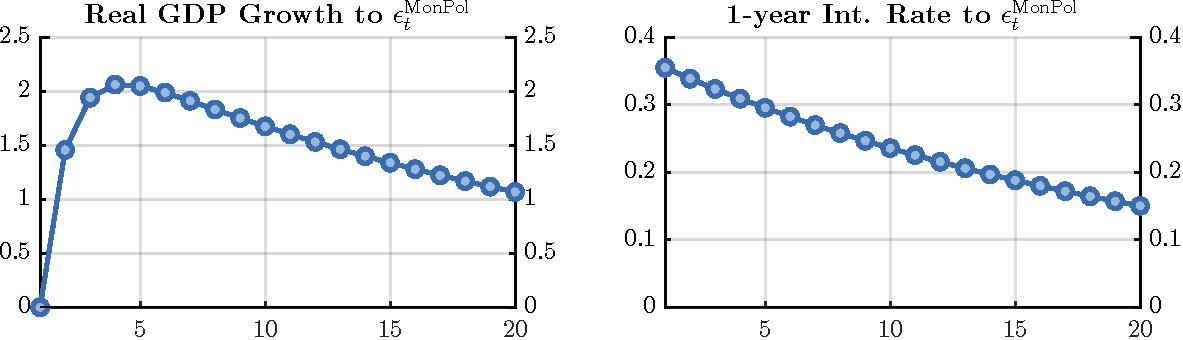
\includegraphics[width=.85\textwidth]{short.pdf}
\end{figure}
\end{frame}
%.......................................................
\shownotesblock{}

%=============================================================
\begin{frame}
\centering
\begin{notebox}[\large \handbold{[BOX]}  \ \textbf{Variable ordering matters!}]{height fill, valign lower=center, segmentation style={draw=notebg}, enlarge left by=-0.25cm, enlarge top by=0.1cm, enlarge bottom by=0.1cm}
\tcblower
\begin{itemize}
\item The \mc{'short'} option assumes $B$ is lower triangular $\Rightarrow$ the ordering of the variables in \mc{X} matters\bigskip
\item The shock in the first equation affects \textit{all} variables on impact; the shock in the second has \textit{zero} contemporaneous effect on the first variable but affects all later ones; and so on\bigskip
\item The ordering encodes an economic assumption: the variable placed first is treated as \textit{causally prior} to all others at the same point in time\bigskip
\item Choose the ordering to be consistent with economic theory and prior intuition
\end{itemize}
\noteboxcenter
\end{notebox}
\end{frame}
%.......................................................
\shownotesblock{}

%=============================================================
\subsection{Zero Long-Run Restrictions}
%=============================================================
\begin{frame}
\color{title}\centering{\huge \textbf{Common Identification Schemes}} \par\bigskip
\color{note}\centering{\Large \textbf{Zero Long-Run Restrictions}}
\end{frame}
%.......................................................
\shownotesblock{}

%=============================================================
\begin{frame}
{Zero long-run restrictions}
\begin{itemize}
\item \textbf{Intuition} \ Identification is achieved by assuming that some shocks have zero cumulative effect on some of the endogenous variables in the long run\bigskip\medskip
\item \textbf{References} \ \cite{BlanchardQuah1989}, \cite{Gali1999}\bigskip
\medskip \pause
\item For example, assume that monetary policy shocks have no long-run effect on the level of output, while supply shocks do \bigskip\medskip\pause
\item But how can we impose restrictions on the long-run cumulative effect of a structural shock?
\end{itemize}
\end{frame}
%.......................................................
\shownotesblock{}

%=============================================================
\begin{frame}
{Zero long-run restrictions}{How to compute the cumulative long-run effects of shocks?}
\begin{itemize}
\item Start from our standard structural VAR representation:%
\begin{equation*}
x_{t}=\Phi x_{t-1}+B\varepsilon_{t}
\end{equation*}%
\pause\smallskip
\item If a shock $\varepsilon_{t}$ hits in $t$, its \textbf{cumulative} impact on $x_{t}$ in the long run is given by
\begin{equation*}
x_{t,t+\infty }={\tikz[tstyle]{\node[nstyle](node1){$B\varepsilon_{t}$};}}+{%
\tikz[tstyle]{\node[nstyle](node2){$\Phi B\varepsilon_{t}$};}}+{%
\tikz[tstyle]{\node[nstyle](node3){$\Phi^{2}B\varepsilon_{t}$};}}+...+\Phi
^{\infty }B\varepsilon_{t}
\end{equation*}%
\pause\smallskip 
\begin{tikzpicture}[tpstyle]
\node[pencil,draw, minimum height=0.6cm, minimum width=0.65cm] (box1) at (node1) {};
\draw[arrow,->,opacity=1] (box1.south) to[bend left] +(-0.9,-0.3) node[gold,anchor=east,opacity=1] {\footnotesize{\textbf{\hand Impact in t}}};
\end{tikzpicture}\pause
\begin{tikzpicture}[tpstyle]
\node[pencil,draw, minimum height=0.6cm, minimum width=0.9cm] (box2) at (node2) {};
\draw[arrow,->,opacity=1] (box2.south) to[bend left] +(-0.1,-0.4) node[gold,anchor=north,opacity=1] {\footnotesize{\textbf{\hand Impact in t+1}}};\end{tikzpicture}%
\pause
\begin{tikzpicture}[tpstyle]
\node[pencil,draw, minimum height=0.6cm, minimum width=1.1cm] (box3) at (node3) {};
\draw[arrow,->,opacity=1] (box3.south) to[bend right] +(+0.1,-0.4) node[gold,anchor=west,opacity=1] {\footnotesize{\textbf{\hand etc...}}};
\end{tikzpicture}\pause\medskip
\item Note: for output growth, $y_{t,t+\infty}$ is the effect of $\varepsilon_t$ on the level of output
\end{itemize}
\end{frame}
%.......................................................
\shownotesblock{}

%=============================================================
\begin{frame}
{Zero long-run restrictions}{How to compute the cumulative long-run effects of shocks?}
\begin{itemize}
\item Re-write the VAR as%
\begin{equation*}
x_{t}=\Phi x_{t-1}+B\varepsilon_{t}
\end{equation*}%
\smallskip
\item If a shock $\varepsilon_{t}$ hits in $t$, its \textbf{cumulative} impact on $x_{t}$ in the long run is given by
\begin{equation*}
x_{t,t+\infty }={\tikz[tstyle]{\node[nstyle](node1){$B\varepsilon_{t}$};}}+{\tikz[tstyle]{\node[nstyle](node2){$\Phi B\varepsilon_{t}$};}}+{\tikz[tstyle]{\node[nstyle](node3){$\Phi^{2}B\varepsilon_{t}$};}}+...+\Phi^{\infty }B\varepsilon_{t}
\end{equation*}%
\smallskip 
\begin{tikzpicture}[tpstyle]
\node[pencil,draw, minimum height=0.6cm, minimum width=0.65cm] (box1) at (node1) {};
\draw[arrow,->,opacity=1] (box1.south) to[bend left] +(-0.9,-0.3) node[gold,anchor=east,opacity=1] {\footnotesize{\textbf{\hand Impact in t}}};
\end{tikzpicture}
\begin{tikzpicture}[tpstyle]
\node[pencil,draw, minimum height=0.6cm, minimum width=0.9cm] (box2) at (node2) {};
\draw[arrow,->,opacity=1] (box2.south) to[bend left] +(-0.1,-0.4) node[gold,anchor=north,opacity=1] {\footnotesize{\textbf{\hand Impact in t+1}}};
\end{tikzpicture}%
\begin{tikzpicture}[tpstyle]
\node[pencil,draw, minimum height=0.6cm, minimum width=1.1cm] (box3) at (node3) {};
\draw[arrow,->,opacity=1] (box3.south) to[bend right] +(+0.1,-0.4) node[gold,anchor=west,opacity=1] {\footnotesize{\textbf{\hand etc...}}};
\end{tikzpicture}\medskip
\item If the VAR is stable, we can rewrite%
\begin{equation*}
x_{t,t+\infty }=\sum\limits_{j=0}^{\infty }\Phi ^{j}B\varepsilon_{t}=\left(I-\Phi \right) ^{-1}B\varepsilon_{t}=C\varepsilon_{t}
\end{equation*}%
where $C\equiv \left( I-\Phi \right) ^{-1}B$ captures the cumulative effect of $\varepsilon_{t}$ on $x_t$ from $t$ to $\infty $
\end{itemize}
\end{frame}
%.......................................................
\shownotesblock{}

%=============================================================
\begin{frame}
{Zero long-run restrictions}{How to compute the cumulative long-run effects of shocks?}
\begin{itemize}
\item What is the intuition for $C$?\bigskip
\item Go back to our output growth / policy rate example. Now assume that the only two shocks driving the economy are a supply and a monetary policy shock:
\begin{equation*}
\begin{bmatrix}
y_{t,t+\infty } \\ 
r_{t,t+\infty }%
\end{bmatrix}%
=\left[ 
\begin{array}{cc}
c_{11} & c_{12} \\ 
c_{21} & c_{22}%
\end{array}%
\right] 
\begin{bmatrix}
\varepsilon_{t}^{Supply} \\ 
\varepsilon_{t}^{MonPol}%
\end{bmatrix}%
\end{equation*}%
\pause
\item Take the first equation: $y_{t,t+\infty }=c_{11}\varepsilon_{t}^{Supply}+c_{12}\varepsilon_{t}^{MonPol}$ \smallskip
\begin{itemize}
\item $c_{12}$ captures the impact of a monetary policy shock (hitting in $t$) on the \lapis{\textbf{level of GDP}} in the long run \smallskip
\item If you believe in long-run monetary neutrality (no long-run effect from monetary policy shocks) you would expect $c_{12}=0$ \medskip
\end{itemize}
\end{itemize}
\end{frame}
%.......................................................
\shownotesblock{}

%=============================================================
\begin{frame}
{Zero long-run restrictions}{How to achieve identification?}
\begin{itemize}
\item Remember that $C\equiv \left( I-\Phi \right) ^{-1}B$ is \lapis{\textbf{unobserved}} as we don't know $B$. \ So, how does this help with the identification of $B$?\bigskip 
\pause
\item To achieve identification define $\Omega \equiv CC^{\prime}$ and note that\smallskip
\begin{enumerate}
\item $\Omega $ is known!%
\begin{equation*}
\Omega =\left( \left( I-\Phi \right) ^{-1}\right) BB^{\prime}\left( \left(
I-\Phi \right) ^{-1}\right) ^{\prime}=\left( \left( I-\Phi \right)
^{-1}\right) \Sigma_{u}\left( \left( I-\Phi \right) ^{-1}\right) ^{\prime}
\end{equation*}%
\pause
\item $\Omega $ is a positive-definite symmetric matrix $\rightarrow$ It admits a unique Cholesky decomposition
\begin{equation*}
\Omega =P_\Omega P_\Omega^{\prime}
\end{equation*}%
\pause\vspace{-0.15cm}
\item Because of our assumption that $C$ is lower triangular, it follows
that $C=P_\Omega$\bigskip \pause
\end{enumerate}
\item We achieved identification: $B=\left( I-\Phi \right) P_\Omega$
\end{itemize}
\end{frame}
%.......................................................
\shownotesblock{}

%=============================================================
\begin{frame}
{Zero long-run restrictions}{How to achieve identification?}
\begin{itemize}
\item As before, we can rewrite the structural VAR with the $B$ matrix implied by the zero long-run restriction
\begin{equation*}
B = (I_2-\Phi)P_\Omega=(I_2-\Phi)
\times \texttt{chol}\left( \left( \left( I-\Phi \right)
^{-1}\right) \Sigma_{u}\left( \left( I-\Phi \right) ^{-1}\right) ^{\prime} \right)
\end{equation*}
where \texttt{chol} denotes the Cholesky factor \bigskip
\pause
\item Note that the $B$ matrix \lapis{\textbf{is not triangular}} \smallskip
\begin{itemize}
\item This is different from what we had in the zero contemporaneous restrictions identification \medskip
\end{itemize}	
\item The impact effects are left unrestricted, the restrictions are on the $C$ matrix \smallskip
\begin{itemize}
\item We'll check later that the restrictions are satisfied in a simple example with true data \medskip
\end{itemize}
\end{itemize}
\end{frame}
%.......................................................
\shownotesblock{}

%=============================================================
\begin{frame}
\centering
\begin{notebox}[\large \handbold{[BOX]}  \ \textbf{The Cholesky decomposition, again}]{height fill, valign lower=center, segmentation style={draw=notebg}, enlarge left by=-0.25cm, enlarge top by=0.1cm, enlarge bottom by=0.1cm}
\tcblower
\begin{itemize}
\item The same Cholesky logic as for zero short-run restrictions applies here, with the long-run matrix $\Omega$ in place of $\Sigma_u$\bigskip
\item Define $\Omega \equiv (I-\Phi)^{-1}\,\Sigma_u\,\big((I-\Phi)^{-1}\big)'$ --- a known, positive-definite, symmetric matrix\bigskip
\item $\Omega$ admits a unique Cholesky factor $P_\Omega$; the lower-triangular structure of $C=(I-\Phi)^{-1}B$ then identifies the system\bigskip
\item As with short-run restrictions, the number of zero restrictions needed grows \textit{faster} than the number of variables --- Cholesky is especially useful as the VAR dimension increases
\end{itemize}
\noteboxcenter
\end{notebox}
\end{frame}
%.......................................................
\shownotesblock{}

%=============================================================
\begin{frame}[fragile]
{Zero long-run restrictions: In Matlab} 
\begin{itemize}
\item Set \mc{VARopt.ident = 'long'} and call \mc{VARmodel} again, saving the results in \mc{VAR\_long}: \par\smallskip
\begin{matlabcode}
% Select zero long-run (Blanchard-Quah) identification
VARopt.ident = 'long';

% Compute impulse responses; plot the MP shock (pick=2)
VAR_long = VARmodel(X,nlags,detc,VARopt);
VARopt.pick = 2;
VARirplot(VAR_long.IR,VARopt);
\end{matlabcode}
\medskip
\item \mc{VAR\_long.B} contains the impact matrix consistent with the zero long-run restrictions \medskip
\item \mc{VAR\_long.IR} contains the impulse responses\medskip
\item Long-run multiplier matrix $C = (I-\Phi)^{-1}B$ can be verified by typing: \mc{(eye(2)-VAR\_long.Fcomp)\textbackslash{}VAR\_long.B}
\end{itemize}
\end{frame}
%.......................................................
\shownotesblock{}

%=============================================================
\begin{frame}
{Zero long-run restrictions: Impulse responses}
\begin{itemize}
\item Monetary policy shock (shock 2) has a zero long-run effect on the output level by construction
\end{itemize}
\begin{figure}[h]
\centering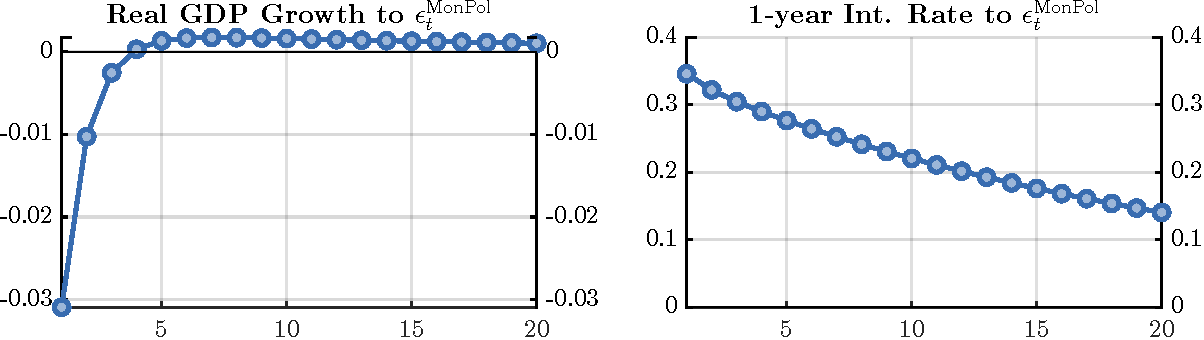
\includegraphics[width=.85\textwidth]{long.pdf}
\end{figure}
\end{frame}
%.......................................................
\shownotesblock{}

%=============================================================
\begin{frame}
{Zero long-run restrictions: Impulse responses}
\smallskip
\begin{itemize}
\item Can also be verified by plotting the cumulative impulse responses over a long-enough horizon \smallskip
\end{itemize}
\begin{figure}[h]
\centering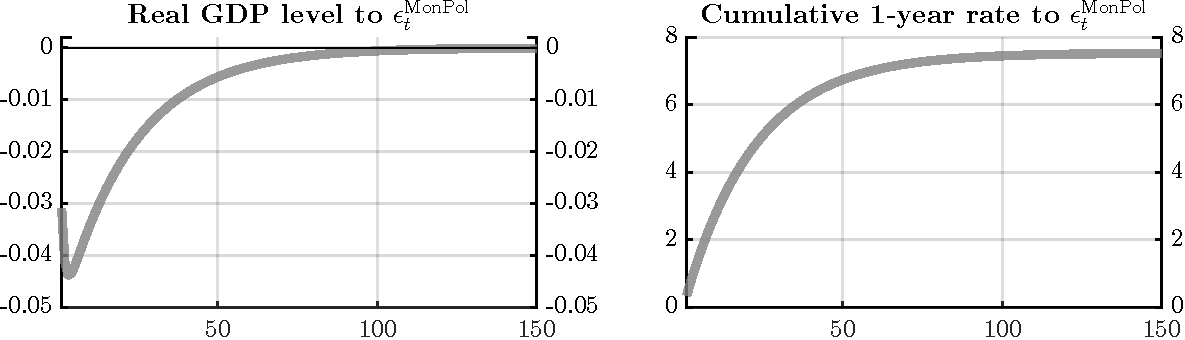
\includegraphics[width=.85\textwidth]{longCum.pdf}
\end{figure}
\end{frame}
%.......................................................
\shownotesblock{}

%=============================================================
\subsection{Sign Restrictions}
%=============================================================
\begin{frame}
\color{title}\centering{\huge \textbf{Common Identification Schemes}}\par\bigskip
\color{note}\centering{\Large \textbf{Sign Restrictions}}
\end{frame}
%.......................................................
\shownotesblock{}

%=============================================================
\begin{frame}
{Sign restrictions}
\begin{itemize}
\item \textbf{Intuition} \ Exploit prior beliefs (typically informed by theoretical models) about the sign that certain\smallskip\ shocks should have on certain endogenous variables\medskip
\item \textbf{Reference} \ \cite{Faust1998}, \cite{CanovaDeNicolo2002}, \cite{Uhlig2005} \medskip \pause		
\item For example \smallskip
\begin{itemize}
\item Demand shocks should lead to an increase in output and interest rates
\smallskip
\item Monetary policy shocks should lead to a fall in output and an increase in interest rates 
\begin{equation*}
\begin{tabular}{lcc}
\hline
\addlinespace 							 & Demand 										& Monetary Policy \\ 	
& ($\varepsilon_{t}^{Demand}$) & ($\varepsilon_{t}^{MonPol}$) \\ \hline\addlinespace 
Output growth ($y_{t}$) 		 & + & - \\ 
Short-rate Int. Rate ($r_{t}$)	 & + & + \\ \hline
\end{tabular}%
\end{equation*}%
\end{itemize}
\pause
\item But how can we impose restrictions on the signs of the effect of a
structural shock?
\end{itemize}
\end{frame}
%.......................................................
\shownotesblock{}

%=============================================================
\begin{frame}
{Sign restrictions}{How to achieve identification?}
\begin{itemize}
\item The key intuition is based on the following three steps\smallskip
\begin{enumerate}
\item Consider a \lapis{\textbf{random orthonormal matrix}} $Q$ such that
\begin{equation*}
QQ^{\prime}=I_{2}
\end{equation*}%
\pause\vspace{-0.15cm}
\item Consider the lower triangular $B$ matrix corresponding to the Cholesky
factor of $\Sigma_{u}$ 
\begin{equation*}
\Sigma_{u}=BB^{\prime}=PP^{\prime}
\end{equation*}%
\pause\vspace{-0.15cm}
\item The following equality holds
\begin{equation*}
\Sigma_{u}=PP^{\prime}=PQQ^{\prime}P^{\prime}=\underset{B}{\underbrace{\left( PQ\right) }}\underset{B^{\prime}}{\underbrace{\left( PQ\right)^{\prime}}}
\end{equation*}%
\pause
\end{enumerate}
\item The matrix $B=PQ$ is a valid `candidate' impact matrix that solves the identification problem! \smallskip
\begin{itemize}
\item Differently from $P$, the matrix $PQ$ is not lower triangular anymore \medskip
\end{itemize}
\end{itemize}
\end{frame}
%.......................................................
\shownotesblock{}

%=============================================================
\begin{frame}
\centering
\begin{notebox}[\large \handbold{[BOX]} \ \textbf{Orthogonal matrix}]{height fill, valign lower=center, segmentation style={draw=notebg}, enlarge left by=-0.25cm, enlarge top by=0.1cm, enlarge bottom by=0.1cm}
\tcblower
\begin{itemize}
\item An orthogonal matrix $Q$ is a real square matrix whose columns form an orthonormal set\bigskip
\item What does it mean? Take for example two $2\times 1$ vectors $q_{1}$ and $q_{2}$, then the matrix $Q=(q_{1},q_{2})$ is orthogonal if \smallskip
\begin{itemize}
\item The vectors have unit norm: $\parallel q_{i}\parallel =1$ \smallskip
\item The vectors are mutually orthogonal: $q_{1}^{T}q_{2}=0$ \medskip
\end{itemize}
\item It follows that
\begin{equation*}
QQ^{\prime}=I \ \ \ \text{and} \ \ \ Q^{\prime}=Q^{-1}
\end{equation*}
\item \textbf{Note} \ You can draw infinite matrices that satisfy the above conditions (we'll see how to do it in Matlab below)
\end{itemize}
\noteboxcenter
\end{notebox}
\end{frame}
%.......................................................
\shownotesblock{}

%=============================================================
\begin{frame}
{Sign restrictions}{How to achieve identification?}
\begin{itemize}
\item But $Q$ is a random matrix... How can we check that $B=PQ$ represents a plausible solution?\medskip \pause
\item \textbf{Solution} \ Check that the effects of shocks implied by $B=PQ$ satisfy a set of a priori sign restrictions. That is:\medskip \pause \smallskip
\begin{itemize}
\item[{[1]}] Consider the structural representation of our VAR%
\begin{equation*}
\left[ 
\begin{array}{c}
y_{t} \\ 
r_{t}%
\end{array}%
\right] =%
\begin{bmatrix}
\phi _{11} & \phi _{12} \\ 
\phi _{21} & \phi _{22}%
\end{bmatrix}%
\left[ 
\begin{array}{c}
y_{t-1} \\ 
r_{t-1}%
\end{array}%
\right] +\left[ 
\begin{array}{cc}
b_{11} & b_{12} \\ 
b_{21} & b_{22}%
\end{array}%
\right] 
\begin{bmatrix}
\varepsilon_{t}^{Demand} \\ 
\varepsilon_{t}^{MonPol}%
\end{bmatrix}%
\end{equation*}%
\pause \smallskip
\item[{[2]}] Then check that the elements of $B$ satisfy\smallskip 
\begin{equation*}
\begin{tabular}{lcc}
\hline
\addlinespace & Demand & Monetary Policy \\ 
& ($\varepsilon_{t}^{Demand}$) & ($\varepsilon_{t}^{MonPol}$) \\ \hline
\addlinespace Output growth ($y_{t}$) & $b_{11}>0$? & $b_{12}<0$? \\ 
Short-rate Int. Rate ($r_{t}$) & $b_{21}>0$? & $b_{22}>0$? \\ \hline
\end{tabular}%
\end{equation*} \medskip
\end{itemize}
\end{itemize}
\end{frame}
%.......................................................
\shownotesblock{}

%=============================================================
\begin{frame}
{Sign restriction in steps}
\begin{itemize}
\item Perform $N$ replications of the following steps \smallskip
\begin{itemize}
\item[{[1]}] Draw a random orthonormal matrix $Q$ \smallskip
\item[{[2]}] Compute $B=PQ$ where $P$ is the Cholesky decomposition of the reduced-form residuals $\Sigma_{u}$ \smallskip
\item[{[3]}] Compute the impact effects of shocks associated with $B$ \smallskip
\item[{[4]}] Are the sign restrictions satisfied? \smallskip
\begin{itemize}
\item[{[4.1]}] Yes. Store $B$ and go back to {\footnotesize \color{title}[1]}
\smallskip
\item[{[4.2]}] No. Discard $B$ and go back to {\footnotesize \color{title}[1]}%
\bigskip \pause \medskip
\end{itemize}
\end{itemize}
\item All matrices in the set $B^{(i)}$ (for $i=1,2,...,N$)\ represent admissible solutions to the identification problem\bigskip
\item In this sense, sign-restricted VARs are only \lapis{\textbf{set identified}}
\end{itemize}
\end{frame}
%.......................................................
\shownotesblock{}

%=============================================================
\begin{frame}
\centering
\begin{notebox}[\large \handbold{[BOX]}  \ \textbf{Set identification vs.\ point identification}]{height fill, valign lower=center, segmentation style={draw=notebg}, enlarge left by=-0.25cm, enlarge top by=0.1cm, enlarge bottom by=0.1cm}
\tcblower
\begin{itemize}
\item \textbf{Point-identified} (Cholesky, long-run) \ A \textit{unique} $B$ satisfies the restrictions. The only source of uncertainty is sampling variability\bigskip
\item \textbf{Set-identified} (sign restrictions) \ \textit{Many} $B_j$ are consistent with the data and the restrictions --- genuinely different structural models, even in an infinite sample\bigskip
\item Consequence 1: the median IRF across draws need not converge to a unique value as $T\to\infty$ --- it summarizes the \textit{set}, not a point estimate\bigskip
\item Consequence 2: credible bands reflect \textit{both} sampling uncertainty \textbf{and} the width of the identified set; the two cannot be disentangled without further restrictions
\end{itemize}
\noteboxcenter
\end{notebox}
\end{frame}
%.......................................................
\shownotesblock{}

%=============================================================
\begin{frame}[fragile]
{Sign restrictions: In Matlab}
\begin{itemize}
\item Encode restrictions in \mc{R} ($+1$ positive, $-1$ negative, $0$ unrestricted)\medskip \item Set \mc{VARopt.ident = 'sign'}, and call \mc{VARmodel} again, saving the results in \mc{VAR\_sr} \par\smallskip
\begin{matlabcode}
% Sign restriction matrix: positive 1, negative -1, unrestricted 0
R = [ 1, -1;  % Real GDP
      1,  1]; % 1-year rate

% Number of random draws and restriction horizon
VARopt.ndraws = 1000;
VARopt.sr_hor = 1;

% Identify with sign restrictions; print acceptance rate as a diagnostic
VARopt.ident = 'sign';
VARopt.R = R;
VAR_sr = VARmodel(X,nlags,detc,VARopt);
\end{matlabcode}
\medskip
\item All accepted draws of the impact matrix stored in \mc{VAR\_sr.Ball} (dimension $2\times 2\times 1000$)
\end{itemize}
\end{frame}
%.......................................................
\shownotesblock{}

%=============================================================
\begin{frame}
{Sign restrictions: Impulse responses}
\begin{itemize}
\item All accepted rotations
\end{itemize}
\begin{figure}[h]
\centering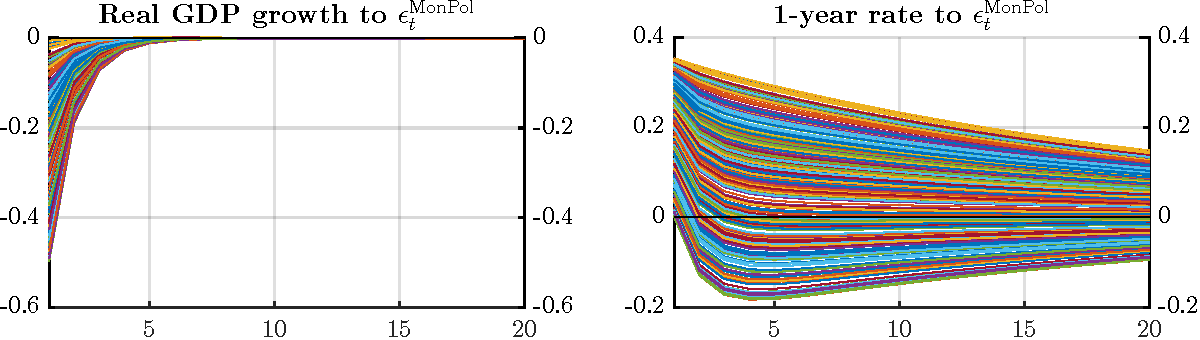
\includegraphics[width=.85\textwidth]{signAll.pdf}
\end{figure}
\end{frame}
%.......................................................
\shownotesblock{}

%=============================================================
\begin{frame}
\centering
\begin{notebox}[\large \handbold{[BOX]}  \ \textbf{Element-wise median vs.\ Fry--Pagan median-target rotation}]{height fill, valign lower=center, segmentation style={draw=notebg}, enlarge left by=-0.25cm, enlarge top by=0.1cm, enlarge bottom by=0.1cm}
\tcblower
\begin{itemize}
\item \textbf{Element-wise median} (\mc{VAR\_sr.IRmed}) \ Coordinate-by-coordinate median across accepted draws. Convenient, but the implied impact matrix \mc{VAR\_sr.Bmed} matches \textit{no} accepted draw and need not satisfy $\Sigma_u = B_{\text{med}}B_{\text{med}}'$ --- a `Frankenstein' object $\Rightarrow$ VD shares need not sum to one, HD need not reproduce the data\bigskip
\item \textbf{Fry--Pagan median-target} (\mc{VAR\_sr.IRfp}) \ The single accepted draw whose responses are closest (least squares) to the element-wise median. A \textit{genuine} structural model: it satisfies the sign restrictions and $\Sigma_u = B_{j^*}B_{j^*}'$ $\Rightarrow$ VD sums to one, HD reproduces the data; cost: it selects one draw from the set\bigskip
\item \textbf{Why they differ} \ Admissible impact matrices lie on a curved set (orthonormal rotations of a Cholesky factor of $\Sigma_u$); the coordinate-wise median generally lies \textit{off} it. Present even with \mc{inference = 0}, and grows with the VAR dimension and the width of the identified set --- hence tiny here (next slide)
\end{itemize}
\noteboxcenter
\end{notebox}
\end{frame}
%.......................................................
\shownotesblock{}

%=============================================================
\begin{frame}
{Sign restrictions: Impulse responses}
\begin{itemize}
\item Median rotation vs.\ Fry--Pagan median-target rotation
\end{itemize}
\begin{figure}[h]
\centering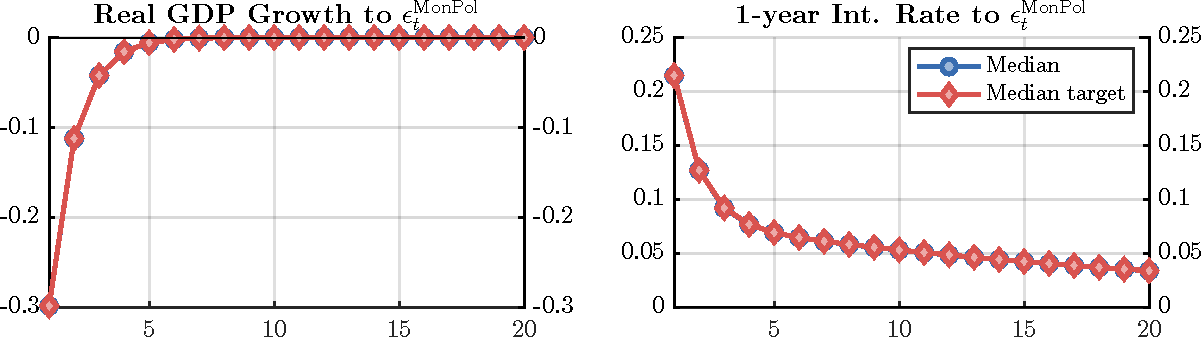
\includegraphics[width=.85\textwidth]{signMed.pdf}
\end{figure}
\end{frame}
%.......................................................
\shownotesblock{}

%=============================================================
\subsection{Narrative Sign Restrictions}
%=============================================================
\begin{frame}
\color{title}\centering{\huge \textbf{Common Identification Schemes}} \par\bigskip
\color{note}\centering{\Large \textbf{Narrative Sign Restrictions}}
\end{frame}
%.......................................................
\shownotesblock{}

%=============================================================
\begin{frame}
{Narrative sign restrictions}
\begin{itemize}
\item \textbf{Intuition} \ Sign restrictions may leave a wide identified set. \textit{Narrative restrictions} exploit well-documented historical episodes to sharpen identification by screening out rotations that are sign-consistent but historically implausible\bigskip \medskip
\item \textbf{References} \ \cite{AntolinDiazRubioRamirez2018}\bigskip \medskip \pause
\item Historical records about specific events carry two types of information \smallskip
\begin{itemize}
\item The \textbf{sign} of a shock at a particular date (e.g.\ the Volcker tightening was a positive MP shock) \smallskip
\item Which shock was the \textbf{dominant driver} of a particular variable at a particular date \medskip
\end{itemize}
\end{itemize}
\end{frame}
%.......................................................
\shownotesblock{}

%=============================================================
\begin{frame}
{Narrative restrictions: Two types}
\begin{itemize}
\item Applied as additional acceptance criteria \textit{after} the sign restrictions are satisfied\bigskip\pause
\item \textbf{\lapis{Type 1} - sign at a date:} \ At date $t^*$, the $m$-th structural shock must have a specified sign
\begin{equation*}
s \cdot \varepsilon_{m,t^*} > 0, \qquad s \in \{+1, -1\}
\end{equation*}\medskip\pause
\item \textbf{\lapis{Type 2} - dominance at a date:} \ At date $t^*$, shock $m$ must account for more of the unexpected movement in variable $i$ than all other shocks combined
\begin{equation*}
\bigl|b_{im}\,\varepsilon_{m,t^*}\bigr| > \sum_{k \neq m} \bigl|b_{ik}\,\varepsilon_{k,t^*}\bigr|
\end{equation*}
where $b_{ik}$ is the $(i,k)$ element of $B$
\end{itemize}
\end{frame}
%.......................................................
\shownotesblock{}

%=============================================================
\begin{frame}
{Narrative sign restrictions in steps}
\begin{itemize}
\item Perform $N$ replications of the following steps \smallskip
\begin{itemize}
\item[{[1]}] Draw a random orthonormal matrix $Q$ \smallskip
\item[{[2]}] Compute $B=PQ$ and check sign restrictions \smallskip
\item[{[3]}] Also check that the implied structural shocks $\varepsilon_t = B^{-1}u_t$ satisfy the narrative restrictions at each specified date $t^*$ \smallskip
\begin{itemize}
\item[{[3.1]}] All restrictions satisfied: retain $B$. Go back to {\footnotesize\color{title}[1]} \smallskip
\item[{[3.2]}] Any restriction violated: discard $B$. Go back to {\footnotesize\color{title}[1]} \medskip
\end{itemize}
\end{itemize}
\item The accepted draws form a \textbf{smaller, differently located set} than sign restrictions alone\bigskip
\item A large decrease in acceptance rate signals that the narrative evidence is genuinely informative
\end{itemize}
\end{frame}
%.......................................................
\shownotesblock{} 

%=============================================================
\begin{frame}[fragile]
{Narrative sign restrictions: In Matlab}
\begin{itemize}
\item Build the \mc{R} (now a structure) with \mc{R.sign}, \mc{R.narr\_sign}, and \mc{R.narr\_dom} \medskip
\item Keep \mc{VARopt.ident='sign'}, call \mc{VARmodel} again, saving the results in \mc{VAR\_nsr} \par\smallskip
\begin{matlabcode}
% Sign restrictions
R.sign = [ 1, -1;  % Real GDP
		   1,  1]; % 1-year rate

% Sign of MP shock for both episodes
R.narr_sign.shock  = [2;        2      ];
R.narr_sign.period = {'1994q1'; '2001q1'};
R.narr_sign.sign   = [1;       -1      ];

% MP shock is the dominant driver of i1yr only in 1994q1
R.narr_dom.shock  = [2;        ];
R.narr_dom.period = {'1994q1'; };
R.narr_dom.var    = [2;        ];

% Identify with sign + narrative restrictions; print acceptance rate as a diagnostic
VARopt.R = R;
VAR_nsr = VARmodel(X, nlags, detc, VARopt);
\end{matlabcode}
\end{itemize}
\end{frame}
%.......................................................
\shownotesblock{}

%=============================================================
\begin{frame}
{Narrative vs.\ Sign-only impulse responses}
\begin{itemize}
\item Narrative restrictions shrink the identified set and shift the median
\end{itemize}
\begin{figure}[h]
\centering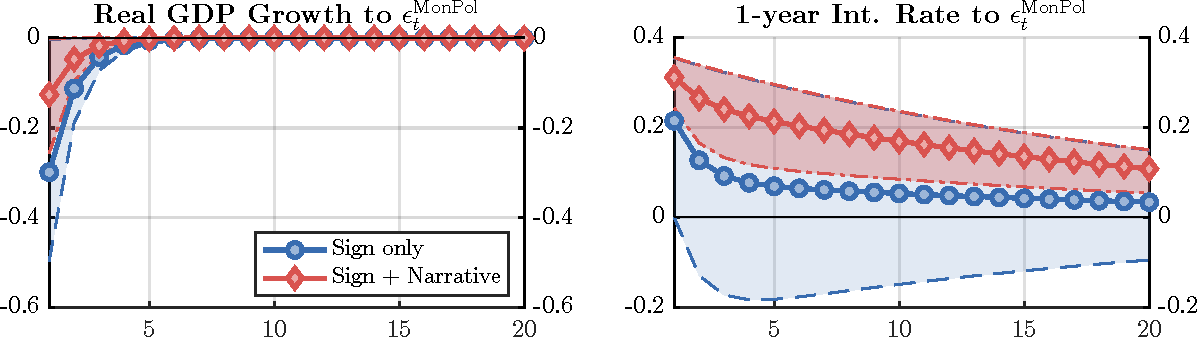
\includegraphics[width=.85\textwidth]{narr.pdf}
\end{figure}
\end{frame}
%.......................................................
\shownotesblock{}

%=============================================================
\begin{frame}
{Narrative vs.\ Sign-only impulse responses}
\begin{itemize}
\item The additional constraints screen out sign-consistent but historically implausible rotations
\end{itemize}
\begin{figure}[h]
\centering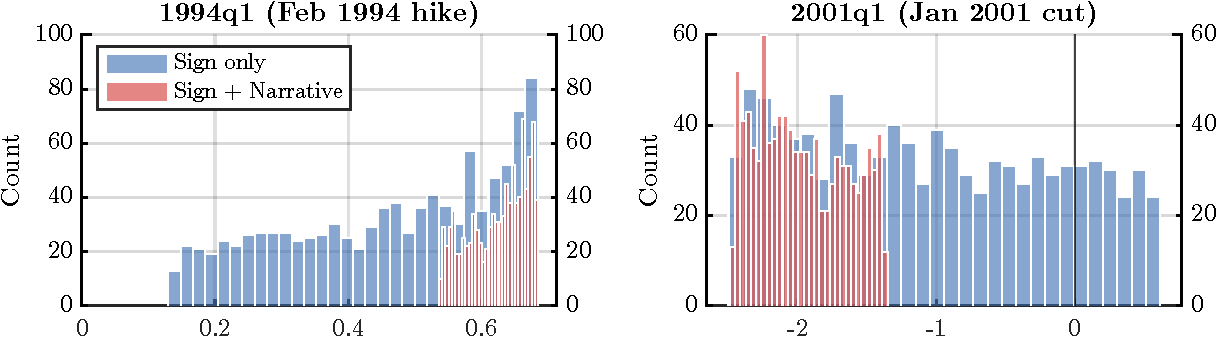
\includegraphics[width=.85\textwidth]{narr_ShockDist.pdf}
\end{figure}
\end{frame}
%.......................................................
\shownotesblock{}




%=============================================================
\subsection{External Instruments}
%=============================================================
\begin{frame}
\color{title}\centering{\huge \textbf{Common Identification Schemes}} \par\bigskip
\color{note}\centering{\Large \textbf{External Instruments (aka Proxy SVARs)}}
\end{frame}
%.......................................................
\shownotesblock{}

%=============================================================
\begin{frame}
{External instruments}
\begin{itemize}
\item \textbf{Intuition} \ Exploit information from a variable that is \emph{external} to the VAR, but that is correlated with a particular shock of interest and uncorrelated with other shocks (the \emph{instrument})\bigskip \medskip
\item \textbf{References} \ \cite{StockWatson2012}, \cite{MertensRavn2013} \bigskip \medskip \pause
\item For example, assume that you have some `narrative' series of policy surprises (i.e. that are not just a response of the central bank to some development in the economy)\bigskip \medskip \pause
\item But how can this help in finding the $B$\ matrix?
\end{itemize}
\end{frame}
%.......................................................
\shownotesblock{}

%=============================================================
\begin{frame}
{External instruments}
\begin{itemize}
\item \textbf{Key element} \ Presence of an \emph{instrument} that is correlated with a shock of interest and uncorrelated with all other shocks \bigskip \medskip \pause
\item For example, assume that such an instrument exists ($z_{t}$) and satisfies the following properties:
\begin{eqnarray*}
\mathbb{E}[\varepsilon_{t}^{Other}z_{t}^{\prime}] &=&0, \\
\mathbb{E}[\varepsilon_{t}^{MonPol}z_{t}^{\prime}] &=&\alpha,
\end{eqnarray*}%
\pause
\item Then, we can identify one column (in this example, the second one) of the $B$ matrix:%
\begin{equation*}
\left[ 
\begin{array}{c}
y_{t} \\ 
r_{t}%
\end{array}%
\right] =%
\begin{bmatrix}
\phi _{11} & \phi _{12} \\ 
\phi _{21} & \phi _{22}%
\end{bmatrix}%
\left[ 
\begin{array}{c}
y_{t-1} \\ 
r_{t-1}%
\end{array}%
\right] +\left[ 
\begin{array}{cc}
- & b_{12} \\
- & b_{22}%
\end{array}%
\right]
\begin{bmatrix}
\varepsilon_{t}^{Other} \\
\varepsilon_{t}^{MonPol}%
\end{bmatrix}%
\end{equation*}
\end{itemize}
\end{frame}
%.......................................................
\shownotesblock{}

%=============================================================
\begin{frame}
{External instruments identification: How does it work?}
\begin{itemize}
\item Recall that the reduced-form residuals are a linear combination of the two structural shocks 
\begin{equation*}
\left\{ 
\begin{array}{c}
u_{yt}=b_{11}\varepsilon_{t}^{Other}+b_{12}\varepsilon_{t}^{MonPol}{\mathbf{%
\medskip }} \\
u_{rt}=b_{21}\varepsilon_{t}^{Other}+b_{22}\varepsilon_{t}^{MonPol}%
\end{array}%
\right.
\end{equation*}%
\vspace{-.2cm}
\item The OLS estimate of $\beta$ in the `first stage' regression identifies $b_{22}$ up to a scaling factor 
\begin{equation*}
u_{rt}=\beta z_{t}+\xi_{t}\pause
\end{equation*}%
\vspace{-.4cm}
\item To see that, recall that the OLS $\beta$ can be written as $\beta = Cov(u_{rt},z_{t})/Var(z_t)$. Focus on the $Cov$ term and plug in the definition of $u_{rt}$ to get 
\begin{equation*}
Cov(u_{rt},z_t)=Cov(b_{21}\varepsilon_{t}^{Other}+b_{22}%
\varepsilon_{t}^{MonPol},z_t)=b_{22}Cov(\varepsilon_{t}^{MonPol},z_t)=
b_{22}\alpha \ \ \jarrowr[len=0.4cm,lw=0.06cm] \ \ \beta = \frac{b_{22}\alpha}{Var(z_t)}
\end{equation*}
\item As $\alpha$ is an unknown constant, $b_{22}=\beta Var(z_t)/\alpha$ is only identified to a scaling factor
\end{itemize}
\end{frame}
%.......................................................
\shownotesblock{}

%=============================================================
\begin{frame}
{External instruments identification: How does it work?}
\begin{itemize}
\item The OLS estimate of $\gamma $ in the following `second stage'
regression identifies the ratio $b_{12}/b_{22}$ 
\begin{equation*}
u_{yt}=\gamma \hat{u}_{rt}+\zeta _{t}=\gamma \left( \frac{b_{22}\alpha}{Var(z_{t})}\right) z_{t}+\zeta _{t}
\end{equation*}%
\vspace{-0.2cm}\pause
\item To see that, and recalling again that $\gamma =Cov(u_{yt},\hat{u}_{rt})/Var(\hat{u}_{rt})$ \smallskip
\begin{itemize}
\item Focus on the $Cov$ term and plug in the definition of $u_{yt}$ and $%
\hat{u}_{rt}$ to get 
\begin{equation*}
Cov(u_{yt},\hat{u}_{rt})=Cov\left( b_{11}\varepsilon_{t}^{Other}+b_{12}\varepsilon _{t}^{MonPol},\frac{b_{22}\alpha}{Var(z_{t})} z_{t}\right) =\frac{b_{12}b_{22}\alpha^{2}}{Var(z_{t})}
\end{equation*}%
\vspace{-0.2cm} \smallskip
\item Then focus on the $Var$ term to get 
\begin{equation*}
Var(\hat{u}_{rt})=Var\left( \frac{b_{22}\alpha}{Var(z_{t})}
z_{t}\right) =\frac{b_{22}^{2}\alpha^{2}}{Var\left( z_{t}\right) }
\end{equation*}%
\vspace{-0.3cm} \smallskip
\item It follows that $\gamma =\frac{b_{12}}{b_{22}}$ \medskip
\end{itemize}
\end{itemize}
\end{frame}
%.......................................................
\shownotesblock{}

%=============================================================
\begin{frame}
{External instruments: Partial identification}
\begin{itemize}
\item In sum, we can normalize the effect of $\varepsilon _{t}^{MonPol}$ on $r_{t}$ to $1$%
\begin{equation*}
b_{22}=1
\end{equation*}
\item And quantify the effect of $\varepsilon _{t}^{MonPol}$ on $y_{t}$ as%
\begin{equation*}
b_{12}=\gamma
\end{equation*}
\item In other words, we have identified the column of the $B$ matrix of the structural VAR\ representation up to a scaling factor
\begin{equation*}
\left[ 
\begin{array}{c}
y_{t} \\ 
r_{t}%
\end{array}%
\right] =%
\begin{bmatrix}
\phi _{11} & \phi _{12} \\ 
\phi _{21} & \phi _{22}%
\end{bmatrix}%
\left[ 
\begin{array}{c}
y_{t-1} \\ 
r_{t-1}%
\end{array}%
\right] +\left[ 
\begin{array}{cc}
- & \gamma \\ 
- & 1%
\end{array}%
\right] 
\begin{bmatrix}
\varepsilon _{t}^{Other} \\ 
\varepsilon _{t}^{MonPol}%
\end{bmatrix}%
\end{equation*}
\smallskip
\begin{itemize}
\item \textbf{Note} It is actually possible to work out the true values of the second column of $B$ (footnote 4 of \cite{GertlerKaradi2015}) \medskip
\end{itemize}
\end{itemize}
\end{frame}
%.......................................................
\shownotesblock{}

%=============================================================
\begin{frame}[fragile]
{External instruments: In Matlab}
\begin{itemize}
\item Pass the instrument via \mc{VARopt.IV} and set \mc{VARopt.ident = 'iv'} \medskip
\item Call \mc{VARmodel} again, saving the results in \mc{VAR\_iv}: 
\par\smallskip
\begin{matlabcode}
% Set identification to 'iv', attach instrument, and compute impulse responses
VARopt.ident    = 'iv';
VARopt.IV       = mps;
VARopt.snames   = {bfeps('MonPol'), bfeps('Other')};
VAR_iv = VARmodel(X,nlags,detc,VARopt);
\end{matlabcode}
\medskip
\item IV-identified column: \mc{VAR\_iv.B(:,1)}; first-stage output in \mc{VAR\_iv.FirstStage}
\end{itemize}
\end{frame}
%.......................................................
\shownotesblock{}


%=============================================================
\begin{frame}
\centering
\begin{notebox}[\large \handbold{[BOX]}  \ \textbf{Warning: the instrument \texttt{mps} is fictitious}]{height fill, valign lower=center, segmentation style={draw=notebg}, enlarge left by=-0.25cm, enlarge top by=0.1cm, enlarge bottom by=0.1cm}
\tcblower
\begin{itemize}
\item \lapisbox[color=BoEred]{\textbf{Warning}} \ The instrument \mc{mps} used in this example is fictitious and must \textit{never} be used in applied work\bigskip
\item A valid instrument needs \textit{relevance} (correlated with the target shock) \textbf{and} \textit{exogeneity} (orthogonal to all other shocks). A canonical example: the high-frequency MP surprises of \cite{GertlerKaradi2015}\bigskip
\item Here \mc{mps} = sign-restriction MP shock $+$ random noise: it makes no economic sense, but works mechanically\bigskip
\item The bivariate VAR(1) is too parsimonious for any real-world instrument --- the example illustrates the \textit{mechanics} of proxy SVARs only
\end{itemize}
\noteboxcenter
\end{notebox}
\end{frame}
%.......................................................
\shownotesblock{}

%=============================================================
\begin{frame}
{External instruments: Impulse responses}
\begin{itemize}
\item Impact responses (stars) from the first/second-stage regressions; dynamic responses from the estimated VAR
\end{itemize}
\begin{figure}[h]
\centering
\includegraphics[width=.85\textwidth]{iv.pdf}
\end{figure}
\end{frame}
%.......................................................
\shownotesblock{}


%=============================================================
\begin{frame}
\centering
\begin{notebox}[\large \handbold{[BOX]}  \ \textbf{Assessing instrument strength: the first-stage $F$-statistic}]{height fill, valign lower=center, segmentation style={draw=notebg}, enlarge left by=-0.25cm, enlarge top by=0.1cm, enlarge bottom by=0.1cm}
\tcblower
\begin{itemize}
\item The first-stage $F$-statistic tests whether the instrument is sufficiently correlated with the reduced-form residual it is meant to instrument\bigskip
\item A \textit{weak} instrument --- low partial correlation with the target --- produces biased and imprecise IV estimates, \textit{regardless} of whether exogeneity holds\bigskip
\item Rule of thumb \citep{StockYogo2002}: the first-stage $F$ should exceed $10$ (one instrument, one regressor, 5\% size-distortion tolerance)\bigskip
\item In the toolbox: \mc{VAR\_iv.FirstStage.F}. \cite{GertlerKaradi2015} report $F$ well above $10$
\end{itemize}
\noteboxcenter
\end{notebox}
\end{frame}
%.......................................................
\shownotesblock{}

%=============================================================
\subsection{Combining Sign Restrictions \& External Instrument}
%=============================================================
\begin{frame}
\color{title}\centering{\huge \textbf{Common Identification Schemes}} \par\bigskip
\color{note}\centering{\Large \textbf{Combining Sign Restrictions \& External Instruments}}
\end{frame}
%.......................................................
\shownotesblock{}

%=============================================================
\begin{frame}
{Combining sign restrictions \& external instruments}
\begin{itemize}
\item \textbf{Intuition} \ Identifies one (or more) columns of $B$ with external instruments and conditional on that the remaining columns with sign restrictions\bigskip \medskip

\item \textbf{References} \ \cite{CesaBianchiSokol2021} \bigskip \medskip \pause

\item For example, assume that there are two shocks that imply similar signs (so that sign restrictions are not enough to identify the shocks), but you have an instrument for
one of the two shocks\bigskip \medskip \pause

\item How can we find the $B$\ matrix?
\end{itemize}
\end{frame}
%.......................................................
\shownotesblock{}

%=============================================================
\begin{frame}
{Combining sign restrictions \& external instruments}
\begin{itemize}
\item Consider a $k$-variable version of our simple structural VAR(1)
\begin{equation*}
\begin{bmatrix}
x_{1t} \\ 
x_{2t} \\ 
\vdots  \\ 
x_{kt}%
\end{bmatrix}%
=\left[ 
\begin{array}{cccc}
\phi _{11} & \phi _{12} & \cdots  & \phi _{1k} \\ 
\phi _{21} & \phi _{22} & \cdots  & \phi _{2k} \\ 
\vdots  & \vdots  & \ddots  & \vdots  \\ 
\phi _{k1} & \phi _{k2} & \cdots  & \phi _{kk}%
\end{array}%
\right] 
\begin{bmatrix}
x_{1t-1} \\ 
x_{2t-1} \\ 
\vdots  \\ 
x_{kt-1}%
\end{bmatrix}%
+\left[ 
\begin{array}{cccc}
b_{11} & b_{12} & \cdots  & b_{1k} \\ 
b_{21} & b_{22} & \cdots  & b_{2k} \\ 
\vdots  & \vdots  & \ddots  & \vdots  \\ 
b_{k1} & b_{k2} & \cdots  & b_{kk}%
\end{array}%
\right] 
\begin{bmatrix}
\varepsilon _{1t} \\ 
\varepsilon _{2t} \\ 
\vdots  \\ 
\varepsilon _{kt}%
\end{bmatrix}%
\end{equation*}
\medskip

\item Assume that \smallskip

\begin{itemize}
\item The first structural shock ($\varepsilon _{1t}$) can be identified with an external instrument \smallskip

\item The remaining structural shocks ($\varepsilon _{2t},...,\varepsilon _{kt}$) can be identified with sign restrictions \medskip
\end{itemize}
\end{itemize}
\end{frame}
%.......................................................
\shownotesblock{}

%=============================================================
\begin{frame}
{Combining sign restrictions \& external instruments}
\begin{itemize}
\item Partition the structural matrix $B$ as $[b \ \mathcal{B}]$
\begin{equation*}
B=\left[ 
\begin{array}{cc}
\underset{b}{\underbrace{%
\begin{array}{c}
b_{11} \\ 
b_{21} \\ 
\vdots  \\ 
b_{k1}%
\end{array}%
}} & \underset{\mathcal{B}}{\underbrace{%
\begin{array}{ccc}
b_{12} & \cdots  & b_{1k} \\ 
b_{22} & \cdots  & b_{2k} \\ 
\vdots  & \ddots  & \vdots  \\ 
b_{k2} & \cdots  & b_{kk}%
\end{array}%
}}%
\end{array}%
\right] 
\end{equation*}
\item Column vector $b$ captures the impact of the first shock, matrix $\mathcal{B}$ captures the impact of the remaining shocks\bigskip 
\item We have seen above how to identify $b$ with external instruments\bigskip 
\item \textbf{Question} Once $b$ is known, how can we find a $\mathcal{B}$ matrix that satisfies a set of sign restrictions?
\end{itemize}
\end{frame}
%.......................................................
\shownotesblock{}

%=============================================================
\begin{frame}
{Combining sign restrictions \& external instruments}
\begin{itemize}
\item Let $P$ be the Cholesky decomposition of $\Sigma_{u}$. Find a normal vector $q$ of dimension $k\times 1$ that rotates the first column of $P$ into the vector $b$, so that
\begin{equation*}
Pq=b
\end{equation*}
\vspace{-0.2cm}
\item Given $q$, build a $(k\times (k-1))$ matrix $\mathcal{Q}$ such that $Q=[q\ \mathcal{Q}]$ is orthonormal%
\begin{equation*}
[q\ \mathcal{Q}][q\ \mathcal{Q}]^{\prime}=QQ^{\prime}=I_k
\end{equation*}
\vspace{-0.2cm}
\item As $Q$ is an orthonormal matrix we have 
\begin{equation*}
\Sigma_{u}=PP^{\prime}=PQQ^{\prime}P^{\prime}=\left( PQ\right) \left(PQ\right) ^{\prime}
\end{equation*}
\vspace{-0.2cm}
\item So $B=PQ$ is a valid candidate matrix that solves the identification problem as \smallskip
\begin{itemize}
\item $\Sigma_{u}=\left( PQ\right) \left(PQ\right) ^{\prime}$ holds \smallskip
\item The first column of $PQ$ is $b$ \medskip
\end{itemize}
\end{itemize}
\end{frame}
%.......................................................
\shownotesblock{}

%=============================================================
\begin{frame}
{Combining sign restrictions \& external instruments: Steps}
\begin{itemize}
\item[{[1]}] Identify $b$, the first column of $B=[b\ \mathcal{B}]$, with the external instrument\medskip 
\item[{[2]}] Compute the Cholesky decomposition $P$ of the reduced-form residuals' covariance matrix $\Sigma_{u}$\medskip
\item[{[3]}] Find a normal vector $q$ that rotates the first column of $P$ into the vector $b$, namely $Pq=b$ \smallskip
\begin{itemize}
\item[{[3.i]}] Given $q$, build the remaining $k-1$ columns of an orthonormal matrix $Q=[q\ \mathcal{Q}]$ \smallskip
\item[{[3.ii]}] The matrix $PQ$ then represents a candidate identification scheme because:
\begin{equation*}
(PQ)(PQ)^{\prime}=\Sigma_{u}\ \ \ \ \ \text{\color{text} and}\ \ \ \ \ P[q\ \mathcal{Q}]=[b\ \mathcal{B}]
\end{equation*}%
\vspace{-0.3cm} \smallskip
\item[{[3.iii]}] If $\mathcal{B}$ satisfies the sign restrictions, retain it. Otherwise, go back to {\color{title!80}[3.i]} \medskip
\end{itemize}
\item[{[4]}] Go back to {\color{title!80}[1]} and repeat $N$ times
\end{itemize}
\end{frame}
%.......................................................
\shownotesblock{}

%=============================================================
\begin{frame}[fragile]
{Combining sign restrictions \& external instruments: In Matlab}
\begin{itemize}
\item Single \mc{VARmodel} call with \mc{ident='sign+iv'}: IV stage pins column~1 of $B$, sign restrictions rotate the orthogonal complement \par\smallskip
\begin{matlabcode}
% Sign restriction for the demand shock (conditional on the IV-identified MP column)
% Positive 1, Negative -1, Unrestricted 0:
R = [ 1;  % Real GDP: positive
1]; % 1-year rate: positive

% Figure path and shock names
VARopt.figname = 'graphics/iv_sign';
VARopt.snames = {bfeps('MonPol'), bfeps('Demand')};

% Run hybrid identification: ident='sign+iv' handles IV stage and sign rotation
% in a single call. VARopt.IV = mps is already set from section 8.
VARopt.ident = 'sign+iv';
VARopt.R = R;
VAR_ivsr = VARmodel(X, nlags, detc, VARopt);
\end{matlabcode}
\medskip
\item IV column fixed at \mc{VAR\_ivsr.Bmed(:,1)} across all draws; median demand-shock responses in \mc{VAR\_ivsr.IRmed}
\end{itemize}
\end{frame}
%.......................................................
\shownotesblock{}

%=============================================================
\begin{frame}
{Combining sign restrictions \& external instruments: Impulse responses}
\begin{itemize}
\item Demand shock responses; MP column is fixed at the IV estimate for every draw
\end{itemize}
\begin{figure}[h]
\centering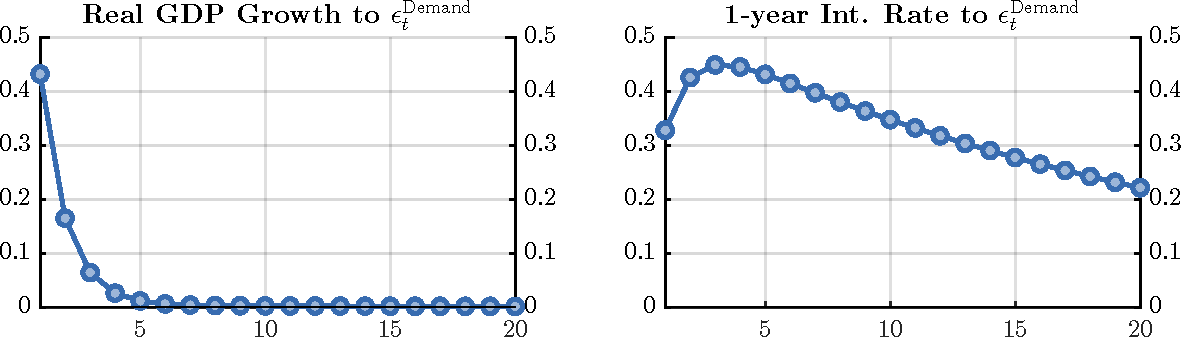
\includegraphics[width=.85\textwidth]{iv_sign.pdf}
\end{figure}
\end{frame}
%.......................................................
\shownotesblock{}

%=============================================================
\subsection{Identification with Exogenous Variables}
%=============================================================
\begin{frame}
\color{title}\centering{\huge \textbf{Common Identification Schemes}} \par\bigskip
\color{note}\centering{\Large \textbf{Identification with Exogenous Variables}}
\end{frame}
%.......................................................
\shownotesblock{}

%=============================================================
\begin{frame}
{Identification with exogenous variables}
\begin{itemize}
\item \textbf{Intuition} \ Suppose you have at your disposal an exogenous shock $s_t$ \smallskip
\begin{itemize}
\item It is \textit{contemporaneously exogenous} to the VAR system \smallskip
\item Rather than using it as an instrument in a second-stage projection \ldots \smallskip
\item \ldots include it \textit{directly} as a contemporaneous regressor in the VAR \medskip
\end{itemize}\pause
\item The model becomes
\begin{equation*}
x_t = c + \sum_{j=1}^{p}\Phi_j x_{t-j} + \delta s_t + u_t
\end{equation*}
where $\delta$ is a $k\times 1$ vector of impact coefficients\bigskip\pause
\item The OLS estimate $\hat{\delta}$, scaled by the sample standard deviation of $s_t$, gives the first column of $B$: the contemporaneous response to a one-standard-deviation shock
\end{itemize}
\end{frame}
%.......................................................
\shownotesblock{}

%=============================================================
\begin{frame}
{Exogenous variables vs.\ Proxy SVAR}
\begin{itemize}
\item Both approaches exploit external variation in the same observed series to identify one structural shock\bigskip\pause
\item The key distinction \smallskip
\begin{itemize}
\item \textbf{Proxy SVAR}: $z_t$ enters as an instrument in a second-stage IV regression on the reduced-form residuals \smallskip
\item \textbf{Exogenous variable}: $s_t$ enters as a contemporaneous regressor \textit{directly} in each VAR equation \medskip
\end{itemize}\pause
\item Under the same identification assumptions and a common lag structure, the two estimators are \textbf{asymptotically equivalent} \ \cite{PlagborgMollerWolf2021}\bigskip
\item Any divergence in finite samples is informative about potential VAR misspecification
\end{itemize}
\end{frame}
%.......................................................
\shownotesblock{}

%=============================================================
\begin{frame}[fragile]
{Identification with exogenous variables: In Matlab}
\begin{itemize}
\item Pass the exogenous shock via \mc{VARopt.exoshock} and set \mc{VARopt.ident = 'exog'} \par\smallskip
\begin{matlabcode}
VARopt_exog = VARoption;
VARopt_exog.vnames    = Xvnames;
VARopt_exog.nsteps    = 20;
VARopt_exog.ident     = 'exog';
VARopt_exog.exoshock  = mps;
VARopt_exog.snames    = {bfeps('MonPol')};
VAR_exog = VARmodel(X, nlags, detc, VARopt_exog);
\end{matlabcode}
\medskip
\item First column of \mc{VAR\_exog.B} equals $\hat{\delta}\hat{\sigma}_s$; remaining columns are zero
\end{itemize}
\end{frame}
%.......................................................
\shownotesblock{}

%=============================================================
\begin{frame}
{Identification with exogenous variables: Impulse responses}
\begin{itemize}
\item Responses virtually identical to the proxy SVAR at all horizons (asymptotic equivalence)
\end{itemize}
\begin{figure}[h]
\centering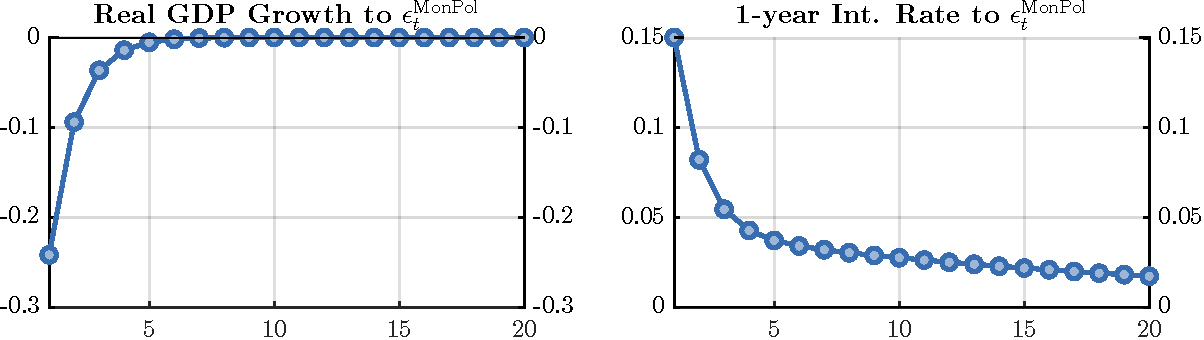
\includegraphics[width=.85\textwidth]{exog.pdf}
\end{figure}
\end{frame}

%=============================================================
\section{Inference}
\begin{frame}
\color{title} \centering{\huge \textbf{Inference}}
\end{frame}
%.......................................................
\shownotesblock{}

%=============================================================
\begin{frame}
{Quantifying uncertainty}
\begin{itemize}
\item Impulse responses, variance decompositions, and historical decompositions are functions of estimated parameters $(\hat{\Phi},\hat{\Sigma}_u)$ --- they inherit sampling uncertainty\bigskip\pause
\item Two distinct situations require different inferential approaches \smallskip
\begin{itemize}
\item \textbf{Point-identified} models (Cholesky, long-run, IV, exogenous): unique $B$; only source of uncertainty is parameter uncertainty $\Rightarrow$ \textbf{bootstrap} \smallskip
\item \textbf{Set-identified} models (sign restrictions, narrative): $B$ is set-identified; uncertainty has two components: parameter uncertainty + identification uncertainty $\Rightarrow$ \textbf{Bayesian draws} \medskip
\end{itemize}
\end{itemize}
\end{frame}
%.......................................................
\shownotesblock{}

%=============================================================
\begin{frame}[fragile]
{Bootstrap for point-identified models}
\begin{itemize}
\item Activate with \mc{VARopt.inference = 1}\bigskip\pause
\item Two variants, selected via \mc{VARopt.method} \smallskip
\begin{itemize}
\item \mc{'bs'} (residual bootstrap): resample residuals with replacement; preserves autocorrelation structure but assumes homoskedastic residuals \smallskip
\item \mc{'wild'}: multiply each residual by an independent $\pm 1$ Rademacher draw; robust to conditional heteroskedasticity; default for proxy SVARs \medskip
\end{itemize}\pause
\begin{matlabcode}
VARopt.inference = 1;       % activate bootstrap
VARopt.method    = 'bs';    % 'bs' = residual bootstrap (default)
VARopt.ndraws    = 1000;    % number of bootstrap draws (default)
VARopt.pctg      = 90;      % confidence level in percent
VAR_id = VARmodel(X, nlags, detc, VARopt);
\end{matlabcode}
\end{itemize}
\end{frame}
%.......................................................
\shownotesblock{}

%=============================================================
\begin{frame}
{Bayesian inference for sign-restricted models}
\begin{itemize}
\item For sign-restricted models, the accepted draws $\{B_j\}$ carry \textbf{both} sources of uncertainty: the rotation draws capture identification uncertainty; an independent draw of VAR parameters from a Normal-inverse-Wishart posterior captures parameter uncertainty\bigskip\pause
\item Control parameter uncertainty via \mc{VARopt.inference} \smallskip
\begin{itemize}
\item \mc{inference = 1} (default): both sources of uncertainty \smallskip
\item \mc{inference = 0}: identification uncertainty only (OLS parameters fixed) \medskip
\end{itemize}\pause
\item Credible bands stored in \mc{VAR\_sr.IRinf} and \mc{VAR\_sr.IRsup}; pointwise median in \mc{VAR\_sr.IRmed} (element-wise median across draws --- not a valid structural model)
\end{itemize}
\end{frame}
%.......................................................
\shownotesblock{}

%=============================================================
\begin{frame}
\centering
\begin{notebox}[\large \handbold{[BOX]}  \ \textbf{Controlling parameter uncertainty in sign-restricted VARs}]{height fill, valign lower=center, segmentation style={draw=notebg}, enlarge left by=-0.25cm, enlarge top by=0.1cm, enlarge bottom by=0.1cm}
\tcblower
\begin{itemize}
\item \mc{VARopt.inference = 1} (default) \ Draws jointly from the posterior over $(\Phi,\Sigma_u)$ \textit{and} over admissible rotations $\Rightarrow$ both parameter \textbf{and} identification uncertainty\bigskip
\item \mc{VARopt.inference = 0} \ Fixes $(\Phi,\Sigma_u)$ at their OLS estimates and randomises only over rotations $\Rightarrow$ identification uncertainty \textit{alone}\bigskip
\item The second setting is useful for isolating the width of the identified set from sampling variability in the reduced-form estimates
\end{itemize}
\noteboxcenter
\end{notebox}
\end{frame}
%.......................................................
\shownotesblock{}

%=============================================================
\section{Dynamic Analysis}
\begin{frame}
\color{title} \centering{\huge \textbf{Dynamic Analysis}}
\end{frame}
%.......................................................
\shownotesblock{}

%=============================================================
\begin{frame}
{Structural dynamic analysis}
\begin{itemize}
\item Assume for the moment that we know how to `identify' structural shocks $\rightarrow$ $B$ matrix is known \bigskip \medskip 
\item What can we do with our structural VAR?\medskip \pause \smallskip
\begin{itemize}
\item Quantify the dynamic effect of a shock over time\ $\Rightarrow $\ \lapis{\textbf{Impulse responses}} \smallskip
\item Quantify how important a shock is in explaining the variation in the endogenous variables (on average)\ $\Rightarrow $\ \lapis{\textbf{Forecast error variance decomposition}} \smallskip
\item Quantify how important a shock was in driving the behavior of the endogenous variables in a specific time period in the past\ $\Rightarrow $\ \lapis{\textbf{Historical decompositions}}\bigskip \medskip
\end{itemize}
\item This is what is called structural dynamic analysis
\end{itemize}
\end{frame}
%.......................................................
\shownotesblock{}

%=============================================================
\subsection{Impulse Responses}
%=============================================================
\begin{frame}
\color{title}\centering{\huge \textbf{Dynamic Analysis}}\par \bigskip
\color{note}\centering{\Large \textbf{Impulse Responses}}
\end{frame}
%.......................................................
\shownotesblock{}

%=============================================================
\begin{frame}
{Impulse response functions}
\begin{itemize}
\item Impulse response functions ($IR$) answer the following question: \par\medskip
\begin{center}
\NB[0.8\textwidth]{What is the response over time of the VAR's endogenous variables to an innovation in the structural shocks, assuming that the other structural shocks are kept to zero?}
\end{center}
\bigskip \medskip \pause
\item $IR$\ allow us to single out the effect of a shock (e.g. its impact and persistence on all variables in the system)\ keeping all else equal\bigskip \medskip
\item \textbf{Example} \ What is the impact of a monetary policy shock to GDP?
\end{itemize}
\end{frame}
%.......................................................
\shownotesblock{}

%=============================================================
\begin{frame}
{How to compute {impulse response functions}}
\begin{itemize}
\item Consider our simple bivariate VAR%
\begin{equation*}
\begin{bmatrix}
y_{t} \\
r_{t}%
\end{bmatrix}%
=%
\begin{bmatrix}
c_{y} \\
c_{r}%
\end{bmatrix}%
+%
\begin{bmatrix}
\phi _{11} & \phi _{12} \\
\phi _{21} & \phi _{22}%
\end{bmatrix}%
\begin{bmatrix}
y_{t-1} \\
r_{t-1}%
\end{bmatrix}%
+%
\begin{bmatrix}
b_{11} & b_{12} \\
b_{21} & b_{22}%
\end{bmatrix}%
\begin{bmatrix}
\varepsilon_{t}^{Demand} \\
\varepsilon_{t}^{MonPol}%
\end{bmatrix}%
\end{equation*}

\item Define a $2\times 1$ impulse selection vector ($s$) that takes value of one for the structural shock that we want to consider.\bigskip

\item For example, to compute the $IR$\ to the demand shock, define $s$ as:%
\begin{equation*}
s=\left[ 
\begin{array}{c}
1 \\ 
0%
\end{array}%
\right]
\end{equation*}

\item The impulse responses to $\varepsilon_{t}^{Demand}$ can be easily
computed with the following equation%
\begin{equation*}
x_{t}=\Phi x_{t-1}+Bs
\end{equation*}
\end{itemize}
\end{frame}
%.......................................................
\shownotesblock{}

%=============================================================
\begin{frame}
{How to compute {impulse response functions (cont'd)}}
\begin{itemize}
\item The $IR$\ can be computed recursively as follows%
\begin{equation*}
\left\{ 
\begin{array}{ll}
IR_{h}=Bs & \ \ \ \ \text{for }h=0 \\
IR_{h}=\Phi IR_{h-1} & \ \ \ \ \text{for }h=1,...,H%
\end{array}%
\right.
\end{equation*}

\item Note that the impact response is simply given by the elements of the impact matrix $B$ selected by $s$...%
\begin{equation*}
\left[ 
\begin{array}{c}
IR_{0}^{y} \\ 
IR_{0}^{r}%
\end{array}%
\right] =\left[ 
\begin{array}{cc}
b_{11} & b_{12} \\ 
b_{21} & b_{22}%
\end{array}%
\right] \left[ 
\begin{array}{c}
1 \\ 
0%
\end{array}%
\right] =\left[ 
\begin{array}{c}
b_{11} \\ 
b_{21}%
\end{array}%
\right]
\end{equation*}

\item ... while the responses at longer horizons are given the transition
matrix 
\begin{equation*}
\left[ 
\begin{array}{c}
IR_{t}^{y} \\ 
IR_{t}^{r}%
\end{array}%
\right] =%
\begin{bmatrix}
\phi _{11} & \phi _{12} \\ 
\phi _{21} & \phi _{22}%
\end{bmatrix}%
\left[ 
\begin{array}{c}
IR_{t-1}^{y} \\ 
IR_{t-1}^{r}%
\end{array}%
\right]
\end{equation*}
\end{itemize}
\end{frame}
%.......................................................
\shownotesblock{}

%=============================================================
\begin{frame}
\centering
\begin{notebox}[\large \handbold{[BOX]} \ \textbf{The companion matrix}]{height fill, valign lower=center, segmentation style={draw=notebg}, enlarge left by=-0.25cm, enlarge top by=0.1cm, enlarge bottom by=0.1cm}
\tcblower
\medskip
\begin{itemize}
\item Every VAR(p) can be written as a VAR(1) using the \textbf{companion representation} \smallskip
\begin{itemize}
\item For example, take a VAR(2)%
\begin{equation*}
\begin{bmatrix}
y_{t} \\
r_{t}%
\end{bmatrix}%
=%
\begin{bmatrix}
c_{y} \\
c_{r}%
\end{bmatrix}%
+%
\begin{bmatrix}
\phi _{11}^{1} & \phi _{12}^{1} \\
\phi _{21}^{1} & \phi _{22}^{1}%
\end{bmatrix}%
\begin{bmatrix}
y_{t-1} \\
r_{t-1}%
\end{bmatrix}%
+%
\begin{bmatrix}
\phi _{11}^{2} & \phi _{12}^{2} \\
\phi _{21}^{2} & \phi _{22}^{2}%
\end{bmatrix}%
\begin{bmatrix}
y_{t-2} \\
r_{t-2}%
\end{bmatrix}%
+%
\begin{bmatrix}
b_{11} & b_{12} \\
b_{21} & b_{22}%
\end{bmatrix}%
\begin{bmatrix}
\varepsilon_{t}^{Demand} \\
\varepsilon_{t}^{MonPol}%
\end{bmatrix}%
\end{equation*} \smallskip
\item Re-write the VAR(2) as%
\begin{equation*}
\left[ 
\begin{array}{c}
y_{t} \\ 
r_{t} \\ 
y_{t-1} \\ 
r_{t-1}%
\end{array}%
\right] ={\tikz[tstyle]{\node[nstyle](node1){$\begin{bmatrix} \phi _{11}^{1}
& \phi _{12}^{1} & \phi _{11}^{2} & \phi _{12}^{2} \\ \phi _{21}^{1} & \phi
_{22}^{1} & \phi _{21}^{2} & \phi _{22}^{2} \\ 1 & 0 & 0 & 0 \\ 0 & 1 & 0 &
0\end{bmatrix}$};}} \left[%
\begin{array}{c}
y_{t-1} \\ 
r_{t-1} \\ 
y_{t-2} \\ 
r_{t-2}%
\end{array}%
\right] +%
\begin{bmatrix}
b_{11} & b_{12} & 0 & 0 \\ 
b_{21} & b_{22} & 0 & 0 \\ 
0 & 0 & 0 & 0 \\ 
0 & 0 & 0 & 0%
\end{bmatrix}%
\begin{bmatrix}
\varepsilon_{t}^{Demand} \\ 
\varepsilon_{t}^{MonPol} \\ 
0 \\ 
0%
\end{bmatrix}%
\end{equation*}
\smallskip
\item Which is a VAR(1) where $\tilde{\Phi}$ is the \textbf{companion matrix}%
\begin{equation*}
\tilde{x}_{t}=\tilde{\Phi}\tilde{x}_{t-1}+\tilde{B}\varepsilon_{t}
\end{equation*} \medskip
\end{itemize}
\end{itemize}
\begin{tikzpicture}[tpstyle]
\node[pencil,draw, minimum height=2.1cm, minimum width=3.35cm] (box1) at (node1) {};
\draw[arrow,->,opacity=1] (box1.north) to[bend left] +(+0.6,+0.3) node[gold,anchor=west,opacity=1] {\footnotesize{\textbf{\hand Companion matrix}}};
\end{tikzpicture}
\end{notebox}
\end{frame}
%.......................................................
\shownotesblock{}

%=============================================================
\begin{frame}[fragile]
{Impulse responses: In Matlab}
\begin{itemize}
\item With identification set, \mc{VARmodel} computes IRFs; \mc{VARirplot} plots them \bigskip
\item Use as an example the sign-restricted VAR from before\bigskip
\item Plot responses to monetary policy shock (shock 2) with confidence bands from the Bayesian posterior\bigskip
\par\smallskip
\begin{matlabcode}
VARopt.inference = 1;       % enable Bayesian credible bands
VAR_sr = VARmodel(X,nlags,detc,VARopt);
VARopt.figname = 'graphics/sign_IR';
VARirplot(VAR_sr.IRmed, VARopt, VAR_sr.IRinf, VAR_sr.IRsup);
\end{matlabcode}
\medskip
\item Growth-rate vs.\ level IRFs: cumulating output growth responses gives the \textbf{output level} response (relevant for long-run neutrality checks)
\end{itemize}
\end{frame}
%.......................................................
\shownotesblock{}

%=============================================================
\begin{frame}
{Impulse responses: Sign-restricted bivariate VAR}
\begin{itemize}
\item Shaded area = 95\% credible bands; solid line = element-wise median
\end{itemize}
\begin{figure}[h]
\centering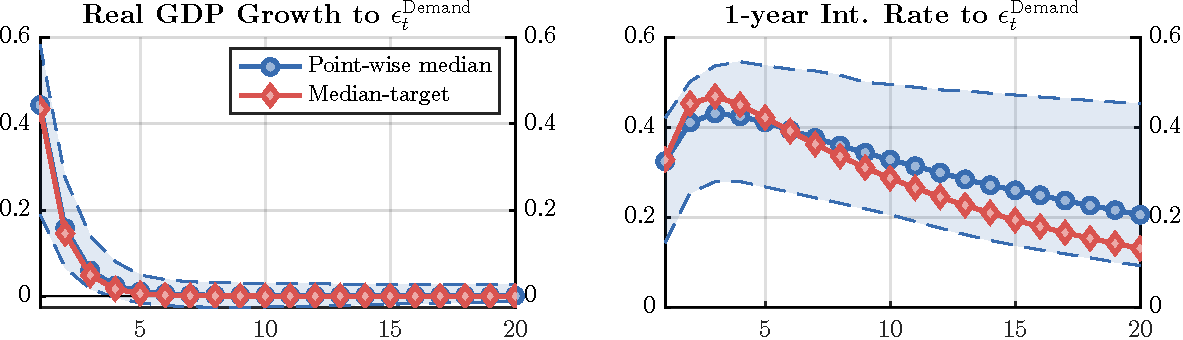
\includegraphics[width=.85\textwidth]{sign_IR_1.pdf}
\end{figure}
\end{frame}
%.......................................................
\shownotesblock{}

%=============================================================
\begin{frame}
\centering
\begin{notebox}[\large \handbold{[BOX]}  \ \textbf{Growth-rate IRFs vs.\ level IRFs}]{height fill, valign lower=center, segmentation style={draw=notebg}, enlarge left by=-0.25cm, enlarge top by=0.1cm, enlarge bottom by=0.1cm}
\tcblower
\begin{itemize}
\item The toolbox computes IRFs for the variables \textit{as they enter the VAR} --- here, the growth rate of GDP. $IR_h^y$ is the deviation of the growth rate from baseline at horizon $h$\bigskip
\item For the \textit{level} of output, the relevant object is the \textbf{cumulative} IRF:
\begin{equation*}
CIR_h^y = \sum_{i=0}^{h} IR_i^y
\end{equation*}
\item The long-run (monetary neutrality) restriction is $CIR_\infty^y = 0$ --- a restriction on the \textit{cumulative} sum, not on any individual growth-rate response\bigskip
\item Growth-rate responses need not return to zero; cumulative (level) responses converge to zero by construction under neutrality
\end{itemize}
\noteboxcenter
\end{notebox}
\end{frame}
%.......................................................
\shownotesblock{}

%=============================================================
\subsection{Forecast Error Variance Decomposition}
%=============================================================
\begin{frame}
\color{title}\centering{\huge \textbf{Dynamic Analysis}} \par \bigskip
\color{note}\centering{\Large \textbf{Forecast Error Variance Decompositions}}
\end{frame}
%.......................................................
\shownotesblock{}

%=============================================================
\begin{frame}
{Forecast error variance decompositions}
\begin{itemize}
\item Forecast error variance decompositions\ ($VD$) answer the following question: \par\medskip
\begin{center}
\NB[0.8\textwidth]{\textit{What portion of the variance of the VAR's forecast errors (at a given horizon $h$) is due to each structural shock?}}
\end{center}
\bigskip \medskip \pause
\item $VD$ provide information about the relative importance of each structural shock in affecting the forecast error variance of the VAR's endogenous variables\bigskip \medskip
\item \textbf{Example} \ What is the (average)\ importance of demand shocks in driving GDP forecast errors?
\end{itemize}
\end{frame}
%.......................................................
\shownotesblock{}

%=============================================================
\begin{frame}
{How to compute {forecast error variance decompositions}}
\begin{itemize}
\item The forecast error of a variable at horizon $t+h$ is the change in the
variable that couldn't have been forecast between $t-1$ and $t+h$ due to the
realization of the structural shocks.\bigskip

\item For example, at $h=0$ we can compute the forecast error as%
\begin{equation*}
x_{t}-\mathbb{E}_{t-1}[x_{t}]=\Phi x_{t-1}+B\varepsilon_{t}-\Phi
x_{t-1}=B\varepsilon_{t}
\end{equation*}

\item At $h=1$, we have 
\begin{eqnarray*}
x_{t+1}-\mathbb{E}_{t-1}[x_{t+1}] &=&\Phi x_{t}+B\varepsilon_{t+1}-\Phi
^{2}x_{t-1}= \\
&=&\Phi (\Phi x_{t-1}+B\varepsilon_{t})+B\varepsilon_{t+1}-\Phi
^{2}x_{t-1}=\Phi B\varepsilon_{t}+B\varepsilon_{t+1}
\end{eqnarray*}

\item So, in general we have 
\begin{equation*}
FE_{t+h}=x_{t+h}-E_{t-1}[x_{t+h}]=\sum_{i=0}^{h}\Phi ^{h-i}B\varepsilon
_{t+i}
\end{equation*}

\item What is the variance of $FE_{t+h}$?
\end{itemize}
\end{frame}
%.......................................................
\shownotesblock{}

%=============================================================
\begin{frame}
\centering
\begin{notebox}[\large \handbold{[BOX]} \ \textbf{Basic properties of the variance}]{height fill, valign lower=center, segmentation style={draw=notebg}, enlarge left by=-0.25cm, enlarge top by=0.1cm, enlarge bottom by=0.1cm}
\tcblower
\begin{itemize}
\item If X is a random variable $x$ and $a$ is a constant \smallskip
\begin{itemize}
\item $Var\left( x+a\right) =Var\left( x\right) $ \smallskip
\item $Var\left( ax\right) =a^{2}Var\left( x\right) $ \medskip
\end{itemize}
\item If $Y$ is a random variable and $b$ is a constant \smallskip
\begin{itemize}
\item $Var\left( aX+bY\right) =a^{2}Var\left( x\right) +b^{2}%
Var\left( Y\right) +2ab Cov\left( X,Y\right) $ \medskip
\end{itemize}
\item Since the structural errors are independent, it follows that $COV\left( \varepsilon_{t+1}^{Demand},\varepsilon_{t+1}^{MonPol}\right) =0$
\end{itemize}
\noteboxcenter
\end{notebox}
\end{frame}
%.......................................................
\shownotesblock{}

%=============================================================
\begin{frame}
{How to compute forecast error variance decompositions (cont'd)}
\begin{itemize}
\item For simplicity consider $h=0$, namely%
\begin{equation*}
Var\left(FE_t\right) = Var\left( x_{t}-E_{t-1}[x_{t}]\right) =Var\left( B\varepsilon
_{t}\right)
\end{equation*}%
\vspace{-.1cm}

\item Recalling that $Var\left( \varepsilon_{t}\right) =I_{2}$ and that the structural shocks are orthogonal to each other, the variance of the forecast error can be computed as%
\begin{eqnarray*}
Var\left( y_{t}-E_{t-1}[y_{t}]\right) &=&b_{11}^{2}Var\left(
\varepsilon_{t}^{Demand}\right) +b_{12}^{2}Var\left( \varepsilon
_{t}^{MonPol}\right) =b_{11}^{2}+b_{12}^{2} \\
Var\left( r_{t}-E_{t-1}[r_{t}]\right) &=&b_{21}^{2}Var\left(
\varepsilon_{t}^{Demand}\right) +b_{22}^{2}Var\left( \varepsilon
_{t}^{MonPol}\right) =b_{21}^{2}+b_{22}^{2}
\end{eqnarray*}%
\vspace{-.1cm}

\item What portion of the variance of the forecast error at $h=0$ is due to
each structural shock? 
\begin{equation*}
\underset{\text{This sums up to 1}}{\underbrace{\left\{ 
\begin{array}{c}
VD_{y_{0}}^{\varepsilon ^{Demand}}=\frac{b_{11}^{2}}{b_{11}^{2}+b_{12}^{2}}%
\medskip \\ 
VD_{y_{0}}^{\varepsilon ^{MonPol}}=\frac{b_{12}^{2}}{b_{11}^{2}+b_{12}^{2}}%
\medskip%
\end{array}%
\right. }}\ \ \ \ \ \ \underset{\text{This sums up to 1}}{\underbrace{%
\left\{ 
\begin{array}{c}
VD_{r_{0}}^{\varepsilon ^{Demand}}=\frac{b_{21}^{2}}{b_{21}^{2}+b_{22}^{2}}%
\medskip \\ 
VD_{r_{0}}^{\varepsilon ^{MonPol}}=\frac{b_{22}^{2}}{b_{21}^{2}+b_{22}^{2}}%
\medskip%
\end{array}%
\right. }}
\end{equation*}
\end{itemize}
\end{frame}
%.......................................................
\shownotesblock{}

%=============================================================
\begin{frame}
{Forecast error variance decomposition: Formula}
\begin{itemize}
\item The VD of variable $i$ at horizon $h$ attributable to shock $j$ is
\begin{equation*}
VD_{i,h}^{\varepsilon^j} = \frac{\sum_{s=0}^{h} (\theta_{ij}^s)^2}{\sum_{s=0}^{h} \sum_{m=1}^{k} (\theta_{im}^s)^2}
\end{equation*}
where $\theta_{ij}^s$ is the $(i,j)$ element of $\Theta_s \equiv \Phi^s B$ (the impulse response matrix at horizon $s$)\bigskip\pause
\item Three properties \smallskip
\begin{itemize}
\item \textbf{Adding-up:} VD shares sum to 1 across shocks at each horizon \smallskip
\item \textbf{Long-run:} as $h\to\infty$, VD converges to the long-run contribution \smallskip
\item \textbf{Identification:} FEVD inherits whatever is recovered by the identification scheme \medskip
\end{itemize}
\end{itemize}
\end{frame}
%.......................................................
\shownotesblock{}
 
%=============================================================
\begin{frame}[fragile]
{FEVD: In Matlab}
\begin{itemize}
\item VD is computed and stored automatically by \mc{VARmodel}, plotted by \mc{VARvdplot} with two `modes' \smallskip
\item Stacked area chart
\begin{matlabcode}
VARopt.figname = 'graphics/sign_VD';
VARvdplot(VAR_sr.VDmed, VARopt);
\end{matlabcode}
\item Line with confidence intervals  
\begin{matlabcode}
VARopt.figname = 'graphics/sign_VD_bands';
VARopt.pick    = 2;
VARopt.color   = pantone('Tomato');
VARvdplot(VAR_sr.VDmed, VARopt, VAR_sr.VDinf, VAR_sr.VDsup);
VARopt.pick    = 0;
VARopt.color   = [];
\end{matlabcode}
\end{itemize}
\end{frame}
%.......................................................
\shownotesblock{}

%=============================================================
\begin{frame}
{FEVD: Sign-restricted bivariate VAR}
\begin{itemize}
\item \textbf{Stacked area}: contribution of each shock to forecast error variance share at every horizon
\end{itemize}
\begin{figure}[h]
\centering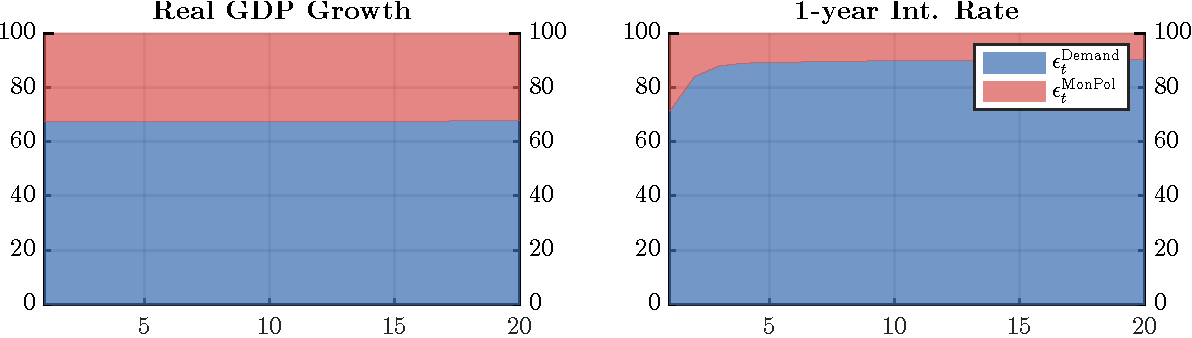
\includegraphics[width=.85\textwidth]{sign_VD.pdf}
\end{figure}
\end{frame}
%.......................................................
\shownotesblock{}

%=============================================================
\begin{frame}
{FEVD: Uncertainty bands}
\begin{itemize}
\item \textbf{Bands}: MP shock contribution with Bayesian credible bands across accepted sign-restriction draws
\end{itemize}
\begin{figure}[h]
\centering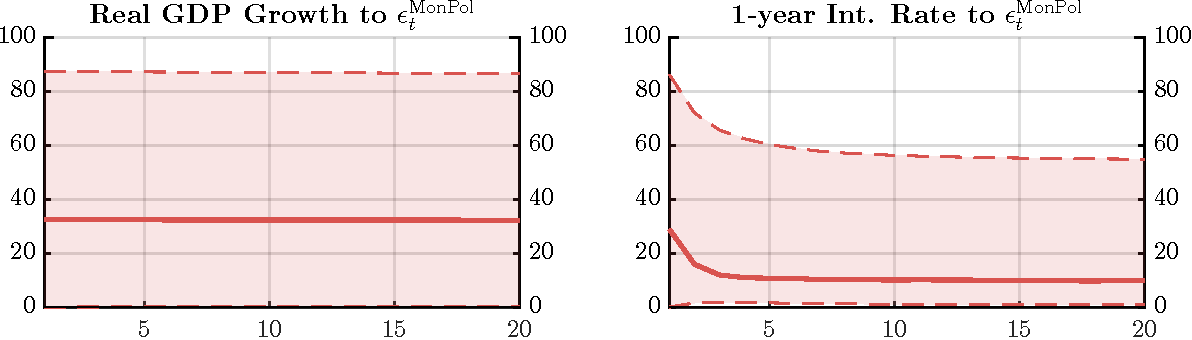
\includegraphics[width=.85\textwidth]{sign_VD_bands.pdf}
\end{figure}
\end{frame}
%.......................................................
\shownotesblock{}

%=============================================================
\begin{frame}
\centering
\begin{notebox}[\large \handbold{[BOX]}  \ \textbf{Three properties of the variance decomposition}]{height fill, valign lower=center, segmentation style={draw=notebg}, enlarge left by=-0.25cm, enlarge top by=0.1cm, enlarge bottom by=0.1cm}
\tcblower
\begin{itemize}
\item \textbf{Adding-up} \ For any variable and horizon, the shares across all $k$ shocks sum to one: $\sum_{j=1}^{k} VD_{y,h}^{\varepsilon^j} = 1$ (under full identification; under partial identification they need not)\bigskip
\item \textbf{Long-run limit} \ For a covariance-stationary VAR, as $h\to\infty$ the FEVD converges to the unconditional variance shares (depending on both $\Phi$ and $B$)\bigskip
\item \textbf{Inherits identification} \ Shares are computed from $\Theta_i = \Phi^i B$, so they depend on the \textit{full} $B$ matrix. Unlike IRFs --- where one column of $B$ suffices --- the FEVD share of shock $j$ requires the full $B$, since the denominator aggregates variance across all $k$ shocks
\end{itemize}
\noteboxcenter
\end{notebox}
\end{frame}
%.......................................................
\shownotesblock{}

%=============================================================
\subsection{Historical Decompositions}
%=============================================================
\begin{frame}
\color{title}\centering{\huge \textbf{Dynamic Analysis}}\bigskip

\color{note}\centering{\Large \textbf{Historical Decompositions}}
\end{frame}
%.......................................................
\shownotesblock{}

%=============================================================
\begin{frame}
{Historical decompositions}
\begin{itemize}
\item Historical decompositions ($HD$) answer the following question:\par\medskip
\begin{center}
\NB[0.8\textwidth]{What is the historical contribution of each structural shock in driving deviations of the VAR's endogenous variables away from their equilibrium?}
\end{center}
\bigskip \medskip \pause
\item $HD$ allow us to track, at each point in time, the role of structural shocks in driving the VAR's endogenous variables away from their steady state\bigskip \medskip
\item \textbf{Example} \ What was the contribution of oil shocks in driving the fall in GDP growth in 1973:Q4?
\end{itemize}
\end{frame}
%.......................................................
\shownotesblock{}

%=============================================================
\begin{frame}
{How to compute historical decompositions }
\begin{itemize}
\item As an example, let's compute the $HD$ of the endogenous variables for $t=2$ in our simple bivariate VAR\bigskip
\item Historical decompositions can be easily understood from the Wold representation of the VAR%
\begin{equation*}
x_{t}={\Phi ^{t}x_{0}}+{\sum\limits_{j=0}^{t-1}\Phi ^{j}c}+{\sum\limits_{j=0}^{t-1}\Phi ^{j}B\varepsilon_{t-j}}
\end{equation*}%
\vspace{-.1cm}\pause
\item Using the Wold representation, we can write $x_{2}$ as a function of present and past structural shocks, the initial condition, and the constant
\begin{equation*}
x_{2}=\underset{init}{\underbrace{\Phi ^{2}x_{0}}}+\underset{const}{\underbrace{(I+\Phi)c}}+\underset{\boldsymbol{\Theta }_{\boldsymbol{1}}}{\underbrace{\Phi B}}\varepsilon_{1}\underset{\boldsymbol{\Theta}_{0}}{+\underbrace{B}}\varepsilon_{2}
\end{equation*}%
\vspace{-.1cm}\pause
\item Re-write $x_{2}$ in matrix form
\begin{equation*}
\begin{bmatrix}
y_{2} \\
r_{2}%
\end{bmatrix}%
=%
\begin{bmatrix}
init_{y} \\
init_{r}%
\end{bmatrix}%
+%
\begin{bmatrix}
const_{y} \\
const_{r}%
\end{bmatrix}%
+%
\begin{bmatrix}
\theta _{11}^{1} & \theta _{12}^{1} \\
\theta _{21}^{1} & \theta _{22}^{1}%
\end{bmatrix}%
\begin{bmatrix}
\varepsilon_{1}^{Demand} \\
\varepsilon_{1}^{MonPol}%
\end{bmatrix}%
+%
\begin{bmatrix}
\theta _{11}^{0} & \theta _{12}^{0} \\
\theta _{21}^{0} & \theta _{22}^{0}%
\end{bmatrix}%
\begin{bmatrix}
\varepsilon_{2}^{Demand} \\
\varepsilon_{2}^{MonPol}%
\end{bmatrix}%
\end{equation*}
\end{itemize}
\end{frame}
%.......................................................
\shownotesblock{}

%=============================================================
\begin{frame}
{How to compute historical decompositions (cont'd)}
\begin{itemize}
\item Then $x_{2}$ can be expressed as
\begin{equation*}
\left\{
\begin{array}{l}
y_{2}=init_{y}+const_{y}+\theta _{11}^{1}\varepsilon_{1}^{Demand}+\theta
_{12}^{1}\varepsilon_{1}^{MonPol}+\theta _{11}^{0}\varepsilon
_{2}^{Demand}+\theta _{12}^{0}\varepsilon_{2}^{MonPol}\medskip \\
r_{2}=init_{r}+const_{r}+\theta _{21}^{1}\varepsilon_{1}^{Demand}+\theta
_{22}^{1}\varepsilon_{1}^{MonPol}+\theta _{21}^{0}\varepsilon
_{2}^{Demand}+\theta _{22}^{0}\varepsilon_{2}^{MonPol}%
\end{array}%
\right.
\end{equation*}%
\pause
\item The historical decomposition is given by 
\begin{equation*}
\begin{array}{ccc}
\underset{\text{This sums up to }y_{2}}{\underbrace{\left\{ 
\begin{array}{l}
HD_{y_{2}}^{\varepsilon ^{Demand}}=\theta _{11}^{1}\varepsilon
_{1}^{Demand}+\theta _{11}^{0}\varepsilon_{2}^{Demand}\medskip \\
HD_{y_{2}}^{\varepsilon ^{MonPol}}=\theta _{12}^{1}\varepsilon
_{1}^{MonPol}+\theta _{12}^{0}\varepsilon_{2}^{MonPol}\medskip \\
HD_{y_{2}}^{init}=init_{y}\medskip \\
HD_{y_{2}}^{const}=const_{y}\medskip%
\end{array}%
\right. }} &  & \underset{\text{This sums up to }r_{2}}{\underbrace{\left\{ 
\begin{array}{l}
HD_{r_{2}}^{\varepsilon ^{Demand}}=\theta _{21}^{1}\varepsilon
_{1}^{Demand}+\theta _{21}^{0}\varepsilon_{2}^{Demand}\medskip \\ 
HD_{r_{2}}^{\varepsilon ^{MonPol}}=\theta _{22}^{1}\varepsilon
_{1}^{MonPol}+\theta _{22}^{0}\varepsilon_{2}^{MonPol}\medskip \\ 
HD_{r_{2}}^{init}=init_{r}\medskip \\
HD_{r_{2}}^{const}=const_{r}\medskip%
\end{array}%
\right. }}%
\end{array}%
\end{equation*}
\end{itemize}
\end{frame}
%.......................................................
\shownotesblock{}

%=============================================================
\begin{frame}[fragile]
{Historical decomposition: In Matlab}
\begin{itemize}
\item HD is computed and stored automatically by \mc{VARmodel}; plot with \mc{VARhdplot} \par\smallskip
\begin{matlabcode}
VARopt.figname = 'graphics/sign_HD';
VARhdplot(VAR_sr.HDmed, VARopt);
\end{matlabcode}
\begin{matlabcode}
VARopt.figname = 'graphics/sign_HD_bands';
VARopt.pick    = 2;
VARopt.color   = pantone('Tomato');
VARhdplot(VAR_sr.HDmed, VARopt, VAR_sr.HDinf, VAR_sr.HDsup);
VARopt.pick    = 0;
VARopt.color   = [];
\end{matlabcode}
\medskip
\item \mc{VAR\_sr.HD} is a struct with fields \mc{shock}, \mc{init}, \mc{const}, \mc{trend}, \mc{endo}
\end{itemize}
\end{frame}
%.......................................................
\shownotesblock{}

%=============================================================
\begin{frame}
{Historical decomposition: Sign-restricted bivariate VAR}
\begin{itemize}
\item Stacked-area: contribution of each shock to the deviation of each variable from its unconditional mean
\end{itemize}
\begin{figure}[h]
\centering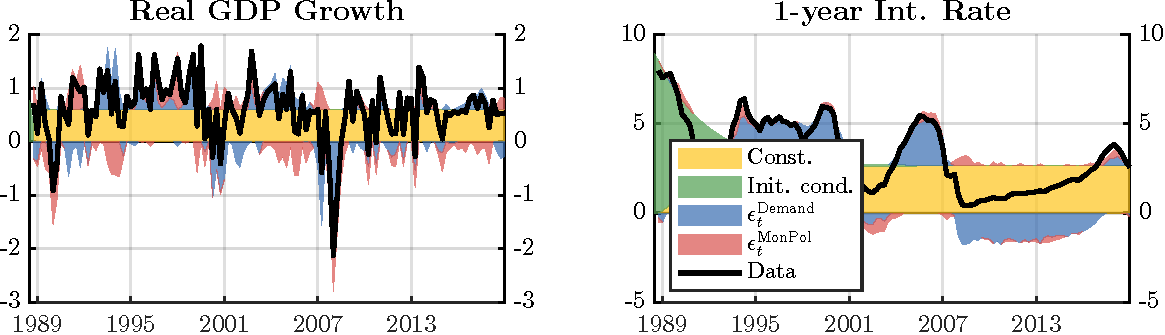
\includegraphics[width=.85\textwidth]{sign_HD.pdf}
\end{figure}
\end{frame}
%.......................................................
\shownotesblock{}

%=============================================================
\begin{frame}
{Historical decomposition: Uncertainty bands}
\begin{itemize}
\item MP shock contribution with Bayesian credible bands; width reflects identification uncertainty across accepted draws
\end{itemize}
\begin{figure}[h]
\centering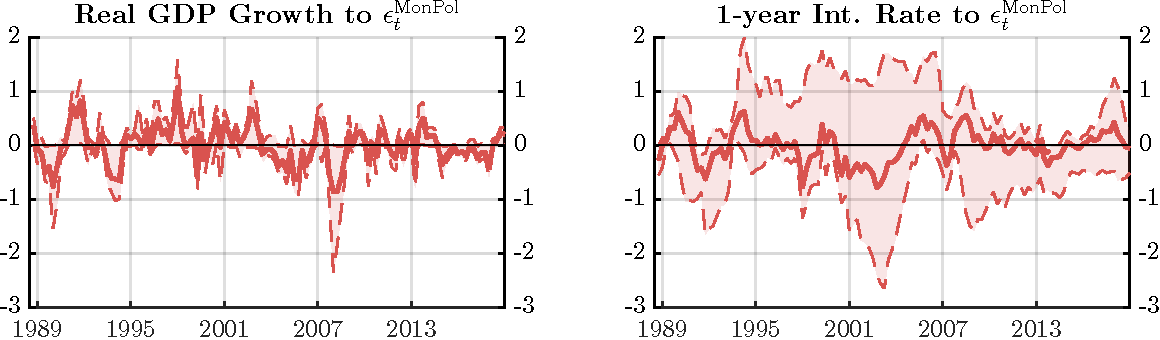
\includegraphics[width=.85\textwidth]{sign_HD_bands.pdf}
\end{figure}
\end{frame}
%.......................................................
\shownotesblock{}

%=============================================================
\begin{frame}
\centering
\begin{notebox}[\large \handbold{[BOX]}  \ \textbf{HD: \texttt{init} and \texttt{const} in log-levels vs.\ log-differences}]{height fill, valign lower=center, segmentation style={draw=notebg}, enlarge left by=-0.25cm, enlarge top by=0.1cm, enlarge bottom by=0.1cm}
\tcblower
\begin{itemize}
\item The economic content of the \mc{init} and \mc{const} components depends on the data transformation\bigskip
\item \textbf{Log-differences VAR} \ The constant converges to the average growth rate (meaningful, stable across samples); the initial condition is the deviation from the long-run average at the sample start, and decays toward zero as the VAR is stable\bigskip
\item \textbf{Log-levels VAR} \ Neither has a stand-alone interpretation: the constant converges to the sample mean of log GDP (grows with the trend, sample-dependent); the initial condition is the first-period log-level, which for a growing economy lies below the mean
\end{itemize}
\noteboxcenter
\end{notebox}
\end{frame}
%.......................................................
\shownotesblock{}

%=============================================================
\section{Local Projections}
\begin{frame}
\color{title} \centering{\huge \textbf{Local Projections}}
\end{frame}
%.......................................................
\shownotesblock{}

%=============================================================
\begin{frame}
{Local projections: Background}
\begin{itemize}
\item \textbf{Intuition} \ Estimate the IRF at each horizon directly \smallskip
\begin{itemize}
\item No fitted VAR to iterate forward \smallskip
\item Regress the $h$-step-ahead outcome on the shock and lagged controls \medskip
\end{itemize}
\item \textbf{Reference} \ \cite{Jorda2005} \medskip\pause
\item One regression per horizon $h = 0, 1, \ldots, H$:
\begin{equation*}
x_{i,t+h} = \alpha_h + \beta_h s_t + \gamma_h' w_t + e_{t+h}
\end{equation*}
\begin{itemize}
\item $\{\hat{\beta}_h\}_{h=0}^H$ traces the response of $x_{i,t+h}$ to $s_t$ \smallskip
\item Std.\ errors: Newey-West HAC, bandwidth $L = h-1$
\end{itemize}
\end{itemize}
\end{frame}
%.......................................................
\shownotesblock{}

%=============================================================
\begin{frame}
{LP vs.\ VAR: Trade-offs}
\begin{itemize}
\item \textbf{Robustness} \ Robust to VAR misspecification \smallskip
\begin{itemize}
\item Each horizon estimated independently, no cross-horizon restrictions \medskip
\end{itemize}\pause
\item \textbf{Efficiency} \ VAR IRFs more efficient when the VAR is correct \smallskip
\begin{itemize}
\item LP fits a separate regression at each horizon \medskip
\end{itemize}\pause
\item \textbf{Equivalence} \ Same population IRFs as the lag order grows \ \cite{PlagborgMollerWolf2021} \medskip
\item \textbf{Complements}, not substitutes \smallskip
\begin{itemize}
\item Divergence at long horizons signals VAR misspecification
\end{itemize}
\end{itemize}
\end{frame}
%.......................................................
\shownotesblock{}

%=============================================================
\begin{frame}[fragile]
{LP-OLS: Estimation in the VAR Toolbox}
\begin{itemize}
\item Pass the full \mc{ENDO} matrix, \mc{LPmodel} loops over its columns (same shock, controls, lags) \smallskip
\item Controls always enter \mc{CTRL} contemporaneously in \mc{LPmodel} 
\begin{itemize}
\item \mc{LPmodel} lags them internally by the pre-specified \mc{nlags}, contemporaneous values never used \medskip
\end{itemize}
\item \mc{mps} (shock $s_t$) and \mc{detc} (deterministic component) carry over from the earlier examples
\par\smallskip
\begin{matlabcode}
% Set up LP-OLS options
LPopt          = LPoption;
LPopt.nsteps   = VARopt.nsteps; % match VAR horizon
LPopt.pctg     = 90;            % 90% confidence bands
LPopt.impact   = 0;             % 1-std-dev shock
LPopt.mnem     = Xmnem;         % mnemonics names
LPopt.vnames   = Xvnames;       % labels for plots
% Run LP-OLS for all endogenous variables in a single matrix call
ENDO = X;   % outcomes x_{i,t+h}
CTRL = X;   % controls w_t (lags constructed internally)
LP = LPmodel(ENDO, mps, CTRL, nlags, detc, LPopt);
\end{matlabcode}
\end{itemize}
\end{frame}
%.......................................................
\shownotesblock{}

%=============================================================
\begin{frame}[fragile]
{LP-IV: Instrumented treatment}
\begin{itemize}
\item When the treatment is endogenous, instrument it via \mc{LPopt.IV}; \smallskip
\begin{itemize}
\item Treatment \mc{ENDO(:,2)} enters as the second argument in \mc{LPmodel} \smallskip
\item \mc{LPopt.IV} holds the external instrument \medskip
\end{itemize}
\item First-stage F-statistic per horizon in \mc{LP\_IV.dlngdp.hN.Fstat\_fs}; check $>10$ (Stock-Yogo threshold)
\par\smallskip
\begin{matlabcode}
%  Set up and run LP-IV
LPopt_IV         = LPoption;
LPopt_IV.nsteps  = VARopt.nsteps;
LPopt_IV.pctg    = 90;
LPopt_IV.impact  = 0;
LPopt_IV.IV      = mps;   % external instrument
LPopt_IV.mnem    = Xmnem; % name per-variable sub-structs
LP_IV = LPmodel(ENDO, ENDO(:,2), CTRL, nlags, detc, LPopt_IV);
\end{matlabcode}
\end{itemize}
\end{frame}
%.......................................................
\shownotesblock{}

%=============================================================
\begin{frame}
{The \texttt{LP} struct}
\begin{itemize}
\item \mc{LPmodel} returns a single struct \mc{LP} \medskip
\begin{itemize}
\item Per-variable sub-structs \mc{LP.dlngdp}, \mc{LP.i1yr} (full univariate output) \smallskip
\item Top-level \mc{IR}, \mc{INF}, \mc{SUP} ($H\times N$): IRFs + Newey-West bands \smallskip
\item Input echo: \mc{ENDO}, \mc{TREAT}, \mc{CTRL}, \mc{EXOG}, \mc{nlag}, \mc{const} \smallskip
\item Per-horizon \mc{h1}, \ldots, \mc{hH}; joint-test fields \mc{jtest\_chi2/df/pval}
\end{itemize}
\end{itemize}
\end{frame}
%.......................................................
\shownotesblock{}

%=============================================================
\begin{frame}
\centering
\begin{notebox}[\large \handbold{[BOX]} \ \textbf{Newey-West standard errors in LP}]{height fill, valign lower=center, segmentation style={draw=notebg}, enlarge left by=-0.25cm, enlarge top by=0.1cm, enlarge bottom by=0.1cm}
\tcblower
\begin{itemize}
\item LP error $e_{t+h}$ = the $h$-step-ahead forecast error \smallskip
\item Under a correct VAR($p$), it is an MA($h-1$):
\begin{equation*}
e_{t+h} = \varepsilon_{t+h} + \psi_1 \varepsilon_{t+h-1} + \cdots + \psi_{h-1}\varepsilon_{t+1}
\end{equation*}
\begin{itemize}
\item Serial correlation up to order $h-1$, even with white-noise $\varepsilon_t$ \medskip
\end{itemize}
\item \textbf{Fix} \ Newey-West HAC, bandwidth $L = h-1$ \smallskip
\begin{itemize}
\item Bands \mc{INF}, \mc{SUP} use \mc{bstd\_NW}
\end{itemize}
\end{itemize}
\noteboxcenter
\end{notebox}
\end{frame}
%.......................................................
\shownotesblock{}

%=============================================================
\begin{frame}
{LP-OLS vs.\ LP-IV: Bivariate example}
\begin{itemize}
\item Both normalized to a 25 bps rise in the 1-year rate on impact \smallskip
\begin{itemize}
\item \textbf{LP-OLS} \ reduced-form effect of an \mc{mps} surprise \smallskip
\item \textbf{LP-IV} \ causal effect of the rate change instrumented by \mc{mps}
\end{itemize}
\end{itemize}
\begin{figure}[h]
\centering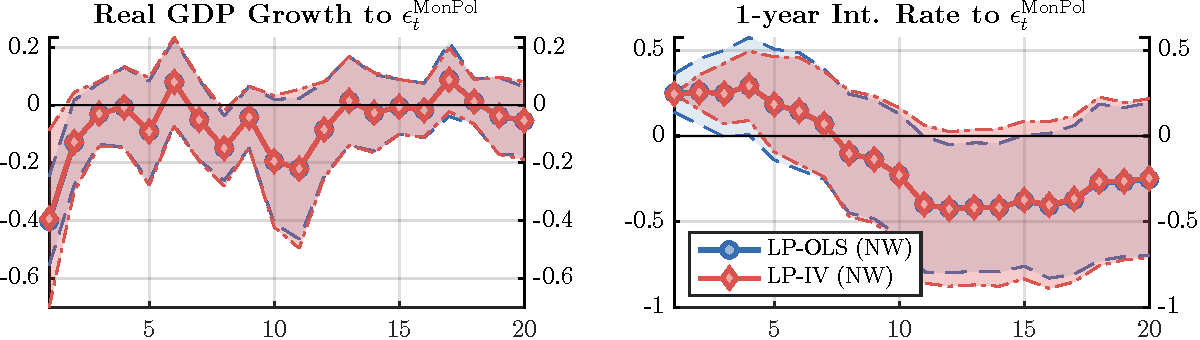
\includegraphics[width=.85\textwidth]{LP_OLS_IV.pdf}
\end{figure}
\end{frame}
%.......................................................
\shownotesblock{}

%=============================================================
\begin{frame}
{LP vs.\ Exogenous-variable SVAR: Two routes to the same object}
\begin{itemize}
\item Recall that LP and the exogenous-variable SVAR are \textbf{the same object} on impact \medskip\pause
\item \textbf{Exog-variable SVAR} \ $s_t$ enters each equation contemporaneously \smallskip
\begin{itemize}
\item Impact identified with the VAR dynamics, then iterated forward \medskip
\end{itemize}
\item \textbf{Local projections} \ project the outcome on $s_t$ at each horizon \smallskip
\begin{itemize}
\item No dynamic model fitted \medskip
\end{itemize}\pause
\item Asymptotically equivalent as the lag order grows \ \cite{PlagborgMollerWolf2021} \smallskip
\begin{itemize}
\item Divergence at $h>0$ signals VAR misspecification
\end{itemize}
\end{itemize}
\end{frame}
%.......................................................
\shownotesblock{}

%=============================================================
\begin{frame}
{LP vs.\ Exogenous-variable SVAR: Bivariate example}
\begin{itemize}
\item Same external instrument, two routes \smallskip
\begin{itemize}
\item \textbf{LP} \ each horizon estimated directly \smallskip
\item \textbf{Exog-SVAR} \ IV-identified impact iterated through the VAR dynamics
\end{itemize}
\end{itemize}
\begin{figure}[h]
\centering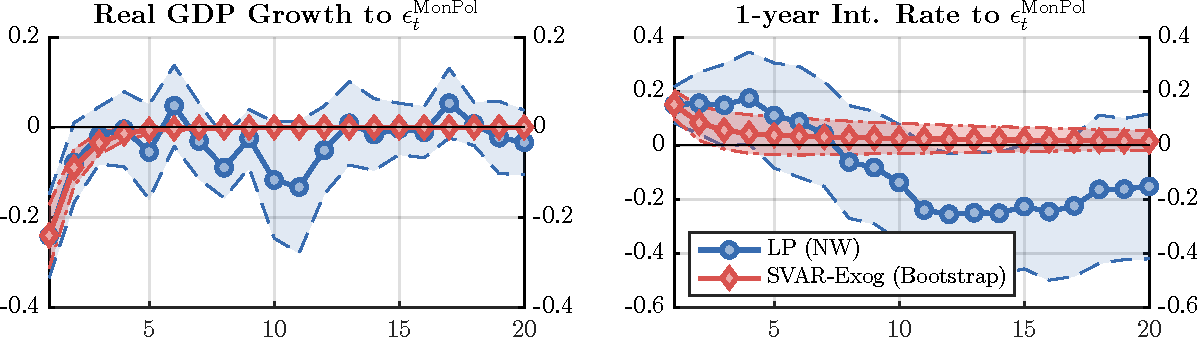
\includegraphics[width=.85\textwidth]{LP.pdf}
\end{figure}
\end{frame}
%.......................................................
\shownotesblock{}

%=============================================================
\appendix
\section{References}
\begin{frame}
\color{title} \centering{\huge \textbf{Appendix}}
\end{frame}
%.......................................................
\shownotesblock{}

%=============================================================
\begin{frame}[allowframebreaks]{References}
\scriptsize
\bibliographystyle{ecta}
\bibliography{BIBLIO.bib}
\end{frame}
%.......................................................
\shownotesblock{}

\end{document}

